\chapter{Introducción}
\label{introduction}

\section{Motivación}

La operación continua, sistemas donde cada una de sus componentes se mantienen operativos todo el tiempo, es un
requerimiento común en muchas aplicaciones. Por lo tanto, es necesario desarrollar técnicas ingenieriles que puedan
actualizar un sistema, tanto su ambiente como sus requerimientos, sin la necesidad de frenar o interrumpir sus
operaciones. Este trabajo ha sido estudiado de diversas maneras, empezando por la actualización dinámica de software
\cite{60317} y más recientemente con el diseño de software adaptable \cite{SEAMS}.

La pregunta central que intenta solucionar este problema es ?`cuándo es seguro cambiar un componente de software en un sistema
que esta corriendo? Una respuesta conservadora a esta pregunta es ``cuando los componentes no están involucrados en
alguna interacción''; esto fue formalizado introduciendo la noción de \textbf{quietud} (\emph{quiescense}) \cite{60317} y luego
\textbf{tranquilidad} (\emph{tranquility}) \cite{4359466}. Muchas otras técnicas han sido desarrolladas (como en
\cite{Anderson:2009:MPM:1656437.1656448} y \cite{485222}) aunque estas nunca explican los requerimientos de
actualización \cite{Baresi:2010:DBD:1882362.1882367}, ni indican cuando es correcto realizar el cambio a la nueva especificación.
Para tal fin Ghezzi et al. \cite{6224401,PanzicaLaManna:2013:FCC:2487336.2487349} estudiaron el problema de actualizar un
controlador que esta monitoreando un ambiente de sistema reactivo mientras controla actuadores. La pregunta que persiguen
contestar los autores es ?`cuándo es seguro reemplazar el controlador actual con uno nuevo, donde se cumple la nueva
especificación?

Un problema en común que los trabajos existentes en actualización dinámica poseen, es que dichas técnicas necesitan
asumir que el sistema que esta siendo ejecutado va a eventualmente alcanzar un estado seguro donde hacer la
actualización. Estos estados son designados como \emph{actualizables} y su identificación depende de cada técnica.
Dichas técnicas, suelen tener un operador o una pieza de software especial designado a identificar dichos estados. Esta asunción, es algo
que no depende del software, sino que depende del ambiente, el cual sabemos que no puede ser manipulado. A su vez, los trabajos
existentes, tampoco dan una técnica para guiar al sistema hacia un estado actualizable. 

Por ejemplo, en \cite{60317}, la expectativa sería que los componentes en un sistema distribuido deben ser diseñados, para que
den información del momento en que dicho componente entró en estado de \emph{quiescence}. A su vez, están diseñados para aceptar mensajes
\emph{pasivate} que, al deshabilitar componentes para inicializar nuevas transacciones, intentan, pero no garantizan
que alcance \emph{quiescence}. Similarmente, en \cite{6224401} requiere asumir que el controlador a ser actualizado va a
volver, eventualmente, a su estado inicial (o asumir que la nueva especificación vale desde el último estado inicial). Estados
actualizables son aquellos en los que el comportamiento del sistema desde el ultimo estado inicial puede controlarse
para satisfacer la nueva especificación.  Por otra parte, en \cite{PanzicaLaManna:2013:FCC:2487336.2487349}, el mismo
autor relaja las condiciones necesarias para realizar una actualización, permitiendo más estados actualizables, al
costo de violar la nueva especificación, y sin contemplar el problema de garantizar que dicho estado sea alcanzado.

%Cuando trabajamos en ingeniería de requerimientos, nuestra tarea es relevar y documentar los objetivos y el
%funcionamiento del ambiente, para elaborar un conjunto de requerimientos cuya máquina a construir debe cumplir.
%Teniendo estas tres componentes, podemos formular la siguiente ecuación: R, D $\vDash$ G. Donde R son los Requerimientos de la
%máquina, D las asunciones del dominio y G los objetivos que la máquina deberá satisfacer.

%Entonces, un problema clave de la ingeniería de requerimientos puede ser visto como un problema de síntesis, tal que
%dado un modelo de la máquina, un modelo del mundo y un conjunto de objetivos del sistema, permite construir un modelo
%operacional el cual satisface los objetivos. La técnica que resuelve esta ecuación mediante los modelos mencionados es
%llamada síntesis de controladores y esta siendo estudiada exhaustivamente en varios aspectos de la ingeniería de los requerimientos.

%La construcción de dichos modelos son una de las principales herramientas en el diseño de sistemas concurrentes, debido
%a que nos facilita la detección de errores de diseño en las primeras etapas de desarrollo. Por otro lado, estos modelos
%de comportamiento pueden resultar complejos de construir. Utilizar la técnica de síntesis anteriormente mencionada
%facilita la construcción tomando modelos pequeños y propiedades lógicas, que suelen ser más sencillas de especificar y de validar.

%Por lo tanto, un problema de control consiste en generar automáticamente una máquina que restrinja la ocurrencia de
%eventos controlables basado en los eventos del mundo que se producen. Es decir, teniendo la especificación de un
%ambiente, asunciones, objetivos y un conjunto de acciones controlables, podemos definir una máquina cuyo comportamiento
%concurrente con el ambiente satisfaga las asunciones y los objetivos del sistema.

%Este problema está siendo ampliamente estudiado en diferentes contextos, desde sistemas autoadaptativos hasta
%composición automática de web-services. Para diseñar softwares autoadaptativos los más evolucionados fueron los basados
%en arquitectura y los basados en requerimientos. El primero de estos utiliza reglas de adaptación que serán utilizadas
%para monitorear condiciones del conjunto de operaciones del sistema y definir acciones en run-time si las condiciones
%son desfavorables. Por otro lado, los basados en requerimientos extienden las técnicas de ingeniería de los
%requerimientos con el fin de representar a los requisitos de adaptación y/o la incertidumbre inherente del medio
%ambiente en el que opera el sistema. El modelo más utilizado en la comunidad, hoy en día, para definir sistemas
%autoadaptables es el modelo arquitectural. 

%Actualmente, trabajos recientes en el área de sistemas auto adaptativos definen una técnica para lograr encontrar
%estados de la ejecución del controlador en los cuales es seguro realizar una actualización y seguir  ejecutando el nuevo
%controlador sin tener que apagar y prender el primero. Sin embargo, dicho problema no ha sido estudiado en el marco de
%síntesis de controladores.

\label{motivation}
\section{Resumen de la contribución}

En esta tesis, como en \cite{6224401,PanzicaLaManna:2013:FCC:2487336.2487349} consideramos el problema de controladores
actualizables en un sistema reactivo. Por otro lado, proponemos una técnica para actualización dinámica que
\emph{fuerza} al sistema a alcanzar un estado actualizable en vez de asumir que el sistema va a llegar a dicho estado.
Por lo tanto, nuestro enfoque no solo garantiza que la nueva especificación va a valer \emph{si} la actualización se
produce, sino que también garantiza que la actualización \emph{va a suceder}. Además, generalizamos la noción de estados
actualizables en \cite{6224401,PanzicaLaManna:2013:FCC:2487336.2487349} mientras mantenemos correctitud que es mejor que
requerir que la nueva especificación empiece a valer desde el estado inicial (o co-inicial 
\cite{PanzicaLaManna:2013:FCC:2487336.2487349}) del controlador actual. Proveemos también una especificación declarativa
y general para señala desde que punto los nuevos objetivos valen y designar propiedades que deben valer en el momento
que el sistema esta transicionando. 

Una clase de sistemas que se amoldan al trabajo presentado son los sistemas adaptables. Dichos sistemas están diseñados
para que, mientras el proceso esta corriendo, pueda soportar cambios en cuanto a la disponibilidad de recursos o
necesidades del usuario y también soportar condiciones inesperadas del ambiente y fallas \cite{SEAMS}. 

Nuestro enfoque de actualización de controladores dinámicos forma parte junto con otros trabajos de la misma área para
síntesis de controladores discretos (ej. \cite{21072}, \cite{Piterman},\cite{D'ippolito:2013:SNE:2430536.2430543}).
Síntesis de controladores automáticamente construye una estrategia operacional (en la forma de máquinas de estado) que
es capaz de garantizar un objetivo bajo asunciones del ambiente.

El problema de controladores dinámicos actualizables puede ser expresado como un problema de síntesis de controladores
en el cual el nuevo controlador cumple que:

\begin{enumerate}[I)]
\item es una estructura equivalente al controlador actual hasta que recibe un mensaje (no controlable) llamado
\emph{beginUpdate},
\item  satisface la especificación actual hasta que el evento (controlable) \emph{stopOldSpec} sucede,
\item garantiza a la nueva especificación desde que ocurre la acción (controlada) \emph{startNewSpec},
\item proporciona que el comportamiento entre \emph{beginUpdate}, \emph{stopOldSpec} y \emph{startNewSpec} satisface
cualquier requerimiento de transición y
\item garantiza que los eventos \emph{startNewSpec} y \emph{stopOldSpec} van a suceder eventualmente.
\end{enumerate}


%Trabajos previos en el área de ingeniería de los requerimientos han estudiado la utilidad de diversas técnicas de sistemas
%adaptativos, debido a la necesidad de cambiar el ambiente o los requerimientos de un sistema sin frenar o interrumpir su
%ejecución.

%La contribución central de esta tesis es la presentación de una técnica que produce la actualización automática de
%sistemas. Dicha técnica, propone mejorar ciertos problemas que las anteriores estrategias padecían, como la necesidad de
%conocer estados de la ejecución en los cuales es ''seguro'' actualizar, y si lo es, detectaremos cual es el estado
%equivalente en el sistema actualizado. Detallaremos en el capitulo BLA por qué y cómo resolvemos dichas complicaciones.

%Por otro lado, lo novedoso del trabajo presentado es el enfoque usado. La actualización automática de sistemas ha sido
%estudiado en diversos enfoques pero no bajo el marco de síntesis de controladores. Al presentar dicha técnica bajo un
%marco no explorado abrimos a la comunidad científica un nuevo paradigma que podría potencialmente solucionar problemas
%en otras áreas relacionadas con la ingeniería de los requerimientos.


\section{Esquema de tesis}

Este trabajo está organizado de la siguiente manera. Empezaremos dando una base de conocimientos teóricos en el capítulo
\ref{background}. Luego de esto, en el capítulo \ref{MTSA_tool} vamos a explicar el soporte que nos da la herramienta
MTSA para poder manejar y controlar todos los conceptos que fueron definidos en el capítulo previo, como el modelado y
la síntesis de controladores.

La técnica central de este trabajo y el aporte científico estará principalmente desarrollado en el capítulo
\ref{updating_controller_chapter}. En éste detallaremos la aplicación de la técnica de síntesis de controladores al
problema de actualización dinámica. Explicaremos además, cómo construimos la solución propuesta y daremos las
definiciones necesarias para finalmente demostrar la correctitud de nuestro enfoque.

En el capítulo \ref{validation}, realizamos un trabajo comparativo entre las técnicas que existen actualmente y la propuesta por
nosotros. Los resultados obtenidos destacando ventajas y desventajas de cada estrategia son expuestos. Explicaremos
además cual es la motivación de utilizar cada caso de estudio.

Finalmente, detallamos los límites y alcances de nuestro trabajo en el capítulo \ref{discusion}. Discutiremos otros
enfoques comparando nuestra labor con trabajos ya existentes. Resaltaremos posibles trabajos futuros que pueden surgir a
partir de este trabajo y concluiremos con un resumen.


\chapter{Fundamentos teóricos}
\label{background}

\section{El Mundo y la Máquina}

Los primeros conceptos que detallaremos estarán involucrados con la ingeniería de los requerimientos. Los puntos de vista
mas relevantes son los de Zave y Jackson (\cite{Zave97fourdark, Jackson:1995:SRA:210207, 5071113}) por un lado, y los de
Letier y Van Lamsweerde (\cite{879820, VanLamsweerde:2001:GRE:882477.883624}) por el otro. Ambos puntos de vista
distinguen a los problemas del \emph{Mundo} y las soluciones de la \emph{Máquina} como fundamentales para reconocer si 
las operaciones de la máquina soluciona los problemas planteados en el mundo. De hecho, el efecto de la máquina en el mundo y las
suposiciones que hacemos acerca de este mundo son fundamentales para el proceso de toma de requerimientos. En el lado
del mundo definimos una serie de problemas que existen en el mundo real que serán solucionados al construir una máquina.
Fácilmente podremos notar que existen componentes en la máquina que interactúan directamente con el mundo siguiendo
normas y procesos conocidos. Estas, forman parte de la intersección entre el mundo y la máquina. Por ejemplo un taladro,
un brazo robótico o las reglas de procesamiento para cada elemento que entra en una linea de producción (ver la Figura
\ref{world_and_machine}).

\begin{figure}
    \centering
    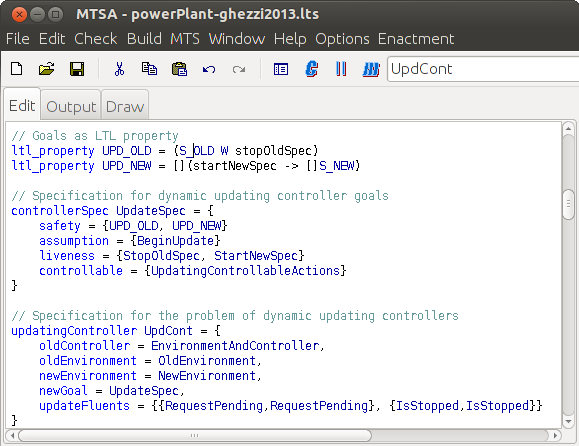
\includegraphics[scale=0.45]{img/MTSA_example.png}
    \caption{El Mundo y la Máquina}
    \label{world_and_machine}
\end{figure}

Así mismo, es esperado que la máquina proponga una solución al problema. Por ejemplo, en la Figura \ref{world_and_machine}
podemos ver que la célula de producción debe procesar cada producto, sólo si están disponible en la bandeja de entrada en ese
momento. Con la sentencia $EnBandeja[p] \rightarrow get.Bandeja[p]$ mostramos que se espera que el brazo del robot sólo
podrá tomar los productos de la bandeja cuando estén listos. Finalizando, los fenómenos compartidos entre el mundo y
máquina, es decir, los que se encuentran en la intersección, representa a la \emph{interfaz}, donde la máquina
interactúa con el mundo. También, podemos definir a los fenómenos del mundo como el \emph{modelo del entorno} ya que el
conjunto de estos describen los eventos que suceden en el mundo real.

Las sentencias que detallan los distintos fenómenos, tanto en el mundo como en la máquina pueden variar en
\emph{alcance} y en \emph{forma} \cite{Parnas95functionaldocuments,Jackson:1995:SRA:210207}. Además, estas pueden estar en modo \emph{indicativo} u \emph{optativo}. En
otros trabajos, como en \cite{van2009requirements}, las sentencias utilizadas son \emph{descriptivas} y \emph{prescriptivas}.

\begin{itemize}
    \item \underline{Sentencias descriptivas:} representan propiedades que son independientes de cómo se comporta el
    sistema. Se usan en modo \emph{indicativo}. No pueden ser cambiadas ni removidas.
    \item \underline{Sentencia prescriptivas:} afirman propiedades deseables que pueden estar presentes o no. Deben estar
    aplicadas por los componentes del sistema. Normalmente, pueden cambiar fortaleciéndose o debilitándose, o incluso
    pueden ser eliminadas. 
\end{itemize}

Anteriormente, fue mencionado que los estados pueden variar en su alcance. Ambos tipos de sentencias pueden referirse a
características de la máquina que no son compartidas por el mundo. En otras ocaciones, sentencias pueden referirse a
fenómenos compartidos por el mundo y la máquina. Más precisamente, una \emph{propiedad de dominio} es
una sentencia descriptiva sobre el mundo. Durante todo este trabajo, vamos a llamar \emph{modelo ambiente}, al conjunto
de propiedades del dominio de un problema particular.

Por otro lado, un \emph{supuesto de ambiente} es una sentencia que podría no suceder y debe ser satisfecha por el
ambiente. Un requisito de software, o \emph{requisito} de forma abreviada, es una sentencia prescriptiva que la máquina
deberá satisfacer independientemente de cómo se comporta el problema detallado en el mundo y deben ser elaboradas en
términos de fenómenos compartidos entre el mundo y la máquina.

Para finalizar y siguiendo lo publicado en \cite{VanLamsweerde:2001:GRE:882477.883624, 879820} podremos determinar a una
acción como supervisada/controlable si dicha acción es supervisada/controlable por la máquina. En este trabajo,
llamaremos a las acciones supervisadas como acciones no controlables, ya que están controladas por el ambiente.

\section{Sistema de Transición Etiquetados (Labelled Transition System)}

En esta sección vamos a dar una notación para los sistemas de transiciones etiquetados o Labelled Transition System
(LTS), la cual usaremos durante este trabajo. Dichos sistemas, son muy usados actualmente para modelar y analizar
comportamiento en sistemas concurrentes y distribuidos. Un LTS es un sistema de transiciones de estados donde cada una
de ellas esta etiquetada con una acción. El conjunto de todas las acciones que posee un LTS es llamado alfabeto.

\begin{nahaDef}
    \emph{(Sistema de Transición Etiquetado)\cite{Keller:1976:FVP:360248.360251} Sea $States$ un conjunto universal de estados, $Act$ un conjunto
    universal de etiquetas. Un Sistema de Transición Etiquetado (LTS) es una tupla $E = (S_E,A_E,\Delta_E,s_{E_0})$,
    donde $S_E \subseteq States$ es un conjunto finito de estados, $A_E \subseteq Act$ es un alfabeto finito, $\Delta_E
    \subseteq (S_E \times A_E \times S_E)$ es una relación, y $s_0 \in S_E$ es el estado inicial.}
\end{nahaDef}

Si $(s,\ell,s') \in \Delta_E$ diremos que $\ell$ está activo desde $s$ en $E$. Diremos también que un LTS $E$ es
\emph{determinístico} si $\forall_{(s,\ell,s'),(s,\ell,s'') \in \Delta_E}$ implica $s' = s''$. Para un estado $s$ definiremos
$\Delta_E(s) = $\{$\ell$ $|$ $(s,\ell,s')$ $\in$ $\Delta_E\}$. Dado un LTS $E$, vamos a referirnos a su alfabeto como $\alpha E$.

\begin{nahaDef}
    \emph{(Composición en Paralelo) Sean $M = (S_M,A_M,\Delta_M, s_{M_0})$ y $E = (S_E,A_E,\Delta_E, s_{E_0})$ LTSs.
    Una Composición en Paralelo($||$) es un operador simétrico tal que $E||M$ es el LTS definido de la siguiente
    manera $E||M = (S_E \times S_M, A_E \cup A_M, \Delta, (s_{E_0},s_{M_0}))$, donde $\Delta$ es la relación mas
    pequeña que satisface las siguientes reglas, donde $\ell \in A_E \cup A_M$:}
\end{nahaDef}

ESCRIBIR GARCHA DE LOGICA

\begin{nahaDef}
    \emph{(LTS Legal) Dado $E = (S_E, A_E, \Delta_E, s_{E_0}), M = (S_M, A_M, \Delta_M, s_{M_0})$ LTSs, y $A_{E_u} \in
    A_E$. Decimos que $M$ es un LTS $Legal$ par $E$ con respecto a $A_{E_u}$ si para todos $(s_E,s_M) \in E||M$ sucede
    lo siguiente: $\Delta_{E||M}((s_E,s_M)) \cap A_{E_u} = \Delta_E(S_E) \cap A_{E_u}$.}
\end{nahaDef} 

Intuitivamente, un LTS $M$ es un LTS $Legal$ para el LTS $E$ con respecto a $A_{E_u}$, si para todos los estados en la
composición $(s_E,s_M) \in S_{S||M}$ se cumple que, una acción $\ell \in A_{E_u}$ es deshabilitada en $(s_E,s_M)$ si y solo
si también esta deshabilitada en $s_E \in E$. En otras palabras, $M$ no restringe a $E$ con respecto a $A_{E_u}$.


\begin{nahaDef}
    \emph{(Tranzas) Sea un LTS $E = (S,A,\Delta,s_0)$. Una secuencia $\pi = \ell_0,\ell_1,...$ es una traza en $E$ si existe una
    secuencia $s_0,\ell_0,s_1,\ell_1,...$ donde para todo $i$ tenemos $(s_i,\ell_i,s_{i+1}) \in \Delta$.}
\end{nahaDef} 


\begin{nahaDef}
    \emph{(Estados Alcanzables) Sea un LTS $E = (S_E, A_E, \Delta_E, s_0)$. Un estado $s \in S_E$ es alcanzable (desde
    el estado inicial) en $E$ si existe una secuencia $s_0,\ell_0,s_1,\ell_1,...$ donde para cada $i$ tenemos
    $(s_i,\ell_i,s_{i+1}) \in \Delta$ y $s = s_{i+1}$. Nos referimos a el conjunto de todos los estados alcanzables en $E$
    como $Reach(E)$.}
\end{nahaDef} 

En el transcurso de esta tesis, vamos a estudiar solo aquellos LTSs $E$ donde todos sus estados $s \in S_E$ son
alcanzables.

\section{Lógica Lineal Temporal de Fluents (Fluent Linear Temporal Logic)}
\label{LTL}

La Lógica Lineal Temporal (LTL) está siendo ampliamente usada en la ingeniería de los requerimientos
\cite{1347546,Giannakopoulou:2003:FMC:940071.940106,879820,Letier:2002:ATG:581339.581353}. La motivación para escoger a
las LTL de fluents es que éstas proveen un framework uniforme para especificar propiedades basados en estados sobre
modelos basados en eventos \cite{Giannakopoulou:2003:FMC:940071.940106}. Fluent Linear Temporal Logic (FLTL) \cite{Giannakopoulou:2003:FMC:940071.940106}
es una lógica de tiempo lineal, temporal, para razonar acerca de fluents. Un \emph{fluent} $Fl$ es definido por un par de
conjuntos y un valor booleano: $Fl = \langle I_{Fl},T_{Fl},Init_{Fl}\rangle$, donde $I_{Fl} \subseteq Act$ es el
conjunto de acciones iniciadoras, $T_{Fl} \subseteq Act$ es el conjunto de acciones finalizadoras y $I_{Fl} \cap T_{Fl}
= \emptyset$. Un fluent puede ser inicializado con valor \emph{true} o \emph{false} indicado por $Init_{Fl}$. Toda acción $\ell \in
Act$ induce un fluent, que notaremos $\ell = \langle\ell, Act \backslash \{\ell\}, false\rangle$. Por último, el alfabeto
de un fluent es el que se obtiene mediante la unión del conjunto de acciones iniciadoras y el conjunto de acciones
finalizadoras.

Sea $\mathcal{F}$ el conjunto de todos los posibles fluents sobre $Act$. Una fórmula FLTL se define inductivamente
utilizando los conectores booleanos estandar y operadores temporales como el $\mathbf{X}$ (próximo), $\mathbf{U}$ (antes
fuerte) de la siguiente manera:

\begin{center}
\begin{equation}
    \varphi ::= Fl\ |\ \neg\varphi\ |\ \varphi\ \lor\ \psi\ |\ \mathbf{X} \varphi\ |\ \varphi\ \mathbf{U}\ \psi
\end{equation}
\end{center}

\noindent donde $Fl \in \mathcal{F}$. Para comodidad sintáctica, vamos a introducir las operaciones de $\land$,
$\Diamond$ (eventualmente) y $\Box$ (siempre). Sea $\Pi$ el conjunto de trazas infinitas sobre $Act$, diremos que la
traza $\pi = \ell_0,\ell_1,...$ satisface un fluent $Fl$ en la posición $i$, notado $\pi,i\vDash Fl$, si y sólo si una de
las siguientes condiciones es válida:

\begin{itemize}
    \item $Init_{Fl} \land (\forall j \in \mathbb{N}: 0 \leq j \leq i \rightarrow \ell_j \notin T_{Fl} )$
    \item $\exists j \in \mathbb{N}: (j \leq i \land \ell_j \in I_{Fl}) \land (\forall k \in \mathbb{N}: j < k \leq i
    \rightarrow \ell_k \notin T_{Fl})$
\end{itemize}

\noindent Dada una traza infinita $\pi$, la fórmula que satisface $\varphi$ en la posición $i$, denotada como $\pi,i
\vDash \varphi$, es definida a continuación como se muestra en la semántica para el operador de satisfacción:

\begin{center}
\begin{tabular}{p{2cm}p{0.5cm}l}
    $\pi,i \vDash \neg\varphi$              & $\triangleq$    & $\neg(\pi,i \vDash \varphi)$\\
    $\pi,i \vDash \varphi \lor \psi$         & $\triangleq$    & $(\pi,i\vDash\varphi)\lor(\pi,i\vDash\psi)$\\
    $\pi,i \vDash \mathbf{X}\varphi$         & $\triangleq$    & $\pi,1 \vDash \varphi$\\
    $\pi,i \vDash \varphi\mathbf{U}\psi$  & $\triangleq$    & $\exists j \geq i: \pi,j \vDash \psi\land\forall i \leq k < j:
    \pi,k \vDash \varphi$
\end{tabular}
\end{center}

Diremos que $\varphi$ se cumple en $\pi$, denotado como $\pi \vDash \varphi$, si $\pi,0 \vDash \varphi$. Una fórmula
$\varphi \in$ FLTL es cierta si un LTS $E$ (denotado como $E \vDash \varphi$) si ésta es cierta en toda traza infinita
producida por $E$. 

\section{Problemas de síntesis de controladores}

Los problemas de síntesis de controladores son aquellos que producen una máquina, la cual, restringe las ocurrencias de
los eventos controlables basado en las observaciones de los eventos no controlados que han ocurridos. Dicha máquina, al
ser desplegada con un ambiente adecuando logramos satisfacer el conjunto de objetivos del sistema. Cabe destacar, que
estos objetivos se cumplirán si se satisfacen las asunciones que se hacen sobre el ambiente. Resumiendo, tendremos una
especificación del ambiente, asunciones, objetivos, y un conjunto de acciones controlables. Resolver el \emph{problema
de síntesis de control} es hallar una máquina, que al trabajar concurrentemente con el ambiente, que satisface las
asunciones del dominio, satisfacemos el conjunto de objetivos del sistema.

Hecha esta introducción definiremos el problema de síntesis de control para modelos basados en eventos de la siguiente
manera. Dada una LTS que detalla el comportamiento del ambiente, un conjunto de eventos controlables, un conjunto de
formulas FLTL que describen los objetivos del sistema, el problema de control LTS consiste en encontrar una LTS que
restringe solamente la ocurrencia de acciones controlables y garantiza que la composición paralela del ambiente con la
LTS recién descripta estará libre de deadlocks y que, si las presunciones del ambiente valen, satisfacerá también los
objetivos del sistema.

\begin{nahaDef}
    \emph{(Control LTS)} Dada una especificación de un entorno en forma de una LTS $E$, un conjunto de acciones
    controlables $A_c \in Act$ y un conjunto $H$ de pares $(A_{s_i}, G_i)$ donde $A_{s_i}$ y $G_i$ son fórmulas FLTL
    especificando presunciones y objetivos del sistema respectivamente, la solución al problema de control LTS
    $\mathcal{E} = <E,H,A_c>$ consiste en encontrar una LTS $M$ de forma que $M$ es legal a $E$ sobre el conjunto de acciones
    no controlables $A_U = \overline{A_c}$, $E||M$ se encuentra libre de deadlocks, y para cada par $(A_{s_i}, G_i) \in
    H$ y para cada traza $\pi$ en $E||M$ se cumple que si $\pi \vDash A_{s_i}$ entonces $\pi \vDash G_i$.
\end{nahaDef}

Como en los tradicionales si


\section{Juegos de dos jugadores}

Llamaremos juegos de dos jugadores a aquellos que consisten en dos jugadores, jugador 1 y jugador 2, donde el objetivo
del jugador 1 es satisfacer una especificación independientemente de las acciones que el jugador 2 ejecute.
Intuitivamente, el jugador 1 puede deshabilitar las acciones que él controla aunque no podrá deshabilitarlas todas ya
que esto transformaría dicho estado a un estado de deadlock.

Durante el transcurso de esta tesis llevaremos los juegos de dos jugadores al marco de síntesis de controladores, donde
el jugador 1 (el controlador) elije, del conjunto de acciones controlables, cual habilitar y el jugador 2 (el ambiente)
elije que acciones tomar libremente. Formalmente podemos definir lo siguiente.

\begin{nahaDef}
    \emph{(Juego de dos jugadores) Un juego de dos jugadores es $G = (S_g, \Gamma^-, \Gamma^+, s_{g_0}, \varphi)$, donde
    $S$ es un conjunto finito de estados, $\Gamma^-, \Gamma^+ \subseteq S \times S$ son conjuntos de transiciones no
    controlables y controlables respectivamente, $s_{g_0} \in S$ es el estado inicial, y $\varphi \subseteq S^\omega$ es
    la condición de ganada. Definimos $\Gamma^-(s) = \{s'\ |\ (s,s') \in \Gamma^-\}$ y análogamente para $\Gamma^+$. Un
    estado $s$ es no controlable si $\Gamma^-(s) \neq \emptyset$ y controlable en el resto de los casos. Una jugada en
    $G$ es una secuencia $p = s_{g_0}, s_{g_1},...$ Una jugada $p$ terminada en $s_{g_n}$ es extendida por el
    controlador eligiendo un subconjunto $\gamma \subseteq \Gamma^+(s_{g_n})$. Luego el ambiente elige un estado
    $s_{g_{n+1}} \in \gamma \cup \Gamma^-(s_{g_n})$ y agrega $s_{g_{n+1}}$ a $p$.}
\end{nahaDef}

Un detalle importante es que si para un estado controlable $\gamma$ el conjunto de opciones del controlador es vacía, esto
puede llevar a un deadlock. Esto será considerado como prohibido mas adelante ya que el controlador definirá este estado
como un estado perdedor. Para un estado no controlable el controlador puede decidir deshabilitar todas las acciones
controlables. Las elecciones del controlador son formalizadas como estrategias y estas reglas son las que el controlador
aplicará. Por lo general, las estrategias son elegidas dependiendo de la historia. Esto puede verse en la estrategia
utilizando un valor de memoria $\Omega$ y actualizando este valor de acuerdo a la evolución del juego.

Es importante destacar, que este tipo de juegos, con memoria, es diferente al definido en \cite{Piterman}. Piterman et al.
define un juego en el cual el ambiente elige su movimiento y recién luego de este, el controlador podrá elegir cual será
el siguiente paso.

\begin{nahaDef}
    \emph{(Estrategia con memoria) Una estrategia con memoria $\Omega$ para el controlador es un par de funciones
    $(\sigma, u)$, donde $\Omega$ es una memoria que tiene designado como valor inicial $\omega_0, \sigma: \Omega \times
    S \rightarrow 2^S$ tal que $\sigma(\omega,s) \subseteq \Gamma^+(s)$ y $u: \Omega \times S \rightarrow \Omega$.}
\end{nahaDef}

Intuitivamente, $\sigma$ le informa al controlador cuales estados debe habilitar como posibles sucesores y $u$ define
como actualizar la memoria en cada paso. Si $\Omega$ es finita, diremos que la estrategia usa memoria finita.

\begin{nahaDef}
    \emph{(Consistencia y estrategia ganadora) una jugada finita o infinita $p = s_0,s_1,...$ es consistente con
    $(\omega,u)$ si para cada $n$ tenemos que $s_{n+1} \in \sigma(\omega_n,s_n)$ donde $\omega_{i+1} =
    u(\omega_i,s_{i+1})$ para toda $i \geq 0$. Una estrategia $(\sigma, u)$ para el controlador desde el estado $s$ es
    ganadora si cada jugada maximal empezando de $s$ y consistente con $(\sigma, u)$ es infinita y en $\varphi$. Diremos
    que el controlador gana el juego $G$ si tiene una estrategia ganadora desde el estado inicial.}
\end{nahaDef}

Diremos que chequear si un controlador gana un juego $G$ es resolver el juego $G$. Una vez definido un juego de dos
jugadores, pasaremos a traducir un problema de síntesis de controladores a este tipo de juegos. La transformación se
basa en generar una estrategia ganadora para el controlador. Si dicha estrategia existe, diremos que el problema de
control es realizable \cite{MalerPS95,21072}. Resultados estudiados anteriormente \cite{Pnueli:1989:SRM:75277.75293},
demuestran que si un controlador gana el juego $G$ y $\varphi$ es $\omega -regular$, el juego puede ganarse utilizando
una estrategia con memoria finita.

\section{Resolviendo el problema de control LTS SGR(1)}

En esta sección explicaremos como una solución para un problema de control SGR(1) puede ser obtenida por construcción
utilizando técnicas existentes de síntesis de controladores (basados en estados), llamados GR(1). \cite{Piterman}

La construcción de la máquina para un problema de control LTS SGR(1) esta divido en dos pasos. Primero, se crea un juego GR(1)
$G$ en representación del ambiente $E$, las asunciones $A_s$, los objetivos $O$ y el conjunto de acciones controlables
$A_C$. Como segundo paso, se elabora una solución $(\sigma,u)$ al juego GR(1) para construir una máquina $M$ (i.e un
controlador LTS) para $\mathcal{E}$. Esta solución al problema de control LTS SGR(1) $\mathcal{E}$ existe, si y solo si,
existe una solución al juego GR(1) $G$. Luego, podremos afirmar que el controlador LTS $M$ creada a partir de
$(\sigma,u)$ es una solución a $\mathcal{E}$.

\subsection{Control LTS SGR(1) a juegos GR(1)}

Convertiremos el problema de control LTS SGR(1) a un juego GR(1). Dado un problema de control LTS SGR(1) $\mathcal{E} =
<E,H,A_C>$ construimos un juego GR(1) $G = (S_g,\Gamma^-,\Gamma^+,s_{g_0},\varphi_g)$ tal que cada estado en $S_g$
representa un estado en $E$ y una valuación de todos los flujos que aparecen en $A_s$ y en $G$.

Mas precisamente, y por la definición de control LTS SGR(1) (definición \ref{ControlLTSSGR1}) tendremos que $H =
\{(\emptyset,I),(A_s,G)\}$, $E = (S_e,A,\Delta_e,s_{e_0})$, $A_s = \bigwedge_{i=1}^n\Box\ \Diamond\ \phi_i$, $I = \Box\
\rho$ y $G = \bigwedge_{j=1}^m\Box\ \Diamond\ \omega_j$. Sea $fl = \{\dot1,...,\dotk\}$ un conjunto de flujos usados en
$A_s$ y en $G$ donde $\doti = <I_i,T_i,Init_i>$. Construimos al juego $G = (S_g,\Gamma^-,\Gamma^+,s_{g_0},\varphi_g)$ de
la siguiente manera.

Construimos $S_g$ a partir de $E$ de tal forma, que los estados en $S_g$ corresponden a un estado en $E$ y los valores
de verdad de los \emph{flujos} en $\varphi$. Formalmente, tenemos que  $S_g = S_e \times \prod_{i=1}^k\{true,false\}$.
Consideramos un estado $s_g = (s_e,\alpha_1,...,\alpha_k)$. Dado un flujo $fl_i$, diremos que $s_g$ satisface $fl_i$ si
$\alpha_i$ es $true$ y $s_g$ no satisface $fl_i$ si no. 

Además, definiremos las relaciones $\Gamma^-$ y $\Gamma^+$ aplicando las siguientes reglas. Sea $s_g =
(s_e,\alpha_1,...,\alpha_k)$. Si $s_g$ no satisface $\rho$ (es decir, $s_g$ es no seguro) no agregaremos los sucesores a
$s_g$. Si $s_g$ satisface $\rho$, por cada transición $(s_e,l,s_e') \in \Delta_e$ agregaremos
$(s_g,(s_e',\alpha_1',...,\alpha_k'))$ en $\Gamma^{\beta}$, donde $\beta$ y $\alpha_i'$ cumplen las siguiente
condiciones:

\begin{center}
\begin{tabular}{ c | c}
$\beta$ & $\alpha_i'$ \\
\hline
es +: si $l \in A_C$, & es $\alpha_i$: si $l \notin I_{fl_i} \cup T_{fl_i}$, \\
es -: si $l \notin A_C$. & es $true$: si $l \in I_{fl_i}$ o \\
& es $false$: si $l \in T_{fl_i}$. \\
\end{tabular}
\end{center}

El estado inicial $s_{g_0}$ es $(s_{e_0},initially_1,...,initially_k)$.

Por último, construiremos la \emph{condición de ganada} $\varphi_g$, definida como un conjunto infinito de trazas, para
$A_S$ y $G$ de la siguiente manera: abusando de la notación denotaremos $\phi_i$ al conjunto de estados $s_g$ tales que
$s_g$ satisface las asunciones $\phi_i$ y a $\gamma_i$ al conjunto de secuencias que satisfacen
$gr((\phi_1,..,\phi_n),(\gamma_1,...,\gamma_m))$. De esta forma, obtendremos que $G = (S_g,\Gamma^-,\Gamma^+,s_{g_0},\varphi_g)$ es un
juego GR(1).

Cabe destacar que las propiedades de seguridad (safety) que son parte de la especificación no están contempladas en la
\emph{condición de ganada} $\varphi_g$ del juego GR(1), pero si se traducen a un problema de \emph{deadlock avoidance} a
la hora de construir $\Gamma^-$ y $\Gamma^+$. De esta manera, la \emph{condicion de ganada} es  $\Box\ \rho
\wedge(\bigwedge_{i=1}^n\Box\Diamond\phi_i \Rightarrow \bigwedge_{j=1}^m \Box\Diamond\omega_j)$.

\subsection{Traduciendo la estrategia a un Controlador LTS}

Ahora pasaremos a explicar como conseguir un controlador LTS a partir de una estrategia ganadora para el juego en GR(1).
Intuitivamente, la transformación es de la siguiente manera: dado un problema de control LTS SGR(1) $\mathcal{E} =
<E,H,A_C>$, el juego $G = (S_g, \Gamma^-, \Gamma^+, s_{g_0},\varphi_g)$ obtenido a partir de $\mathcal{E}$ y de la
estrategia ganadora para $G$, construimos $M = (S_M,A,\Delta_M,s_{M_0})$ una solución para $\mathcal{E}$ traduciendo
a estados de $S_M$ un estado de $S_g$ y un estado de la memoria dada por la estrategia ganadora.

Mas formalmente, sea $E = (S_e,A,\Delta_e,s_{e_0})$, $fl = \{fl_1,...,fl_k\}$ el conjunto de flujos que aparecen en
$\varphi$, $G = (S_g,\Gamma^-,\Gamma^+,s_{g_0},\varphi_g)$ el juego GR(1) construido a partir de $E$ como explicamos
anteriormente, y sea $\sigma: \Omega \times S_g \rightarrow 2^{S_g}$ y $u: \Omega \times S_g \rightarrow \Omega$ la
estrategia ganadora para $G$. Construiremos la máquina $M = (S_M, A, \Delta_M, s_{M_0})$ de la siguiente manera.

Para construir $S_M \subseteq \Omega \times S_g$, consideremos dos estados $s_g = (s_e,\alpha_1,...,\alpha_k)$ y $s_g' =
(s_e',\alpha_1',...,\alpha_k')$. Decimos que esa acción $\ell$ es \emph{posible} desde $s_g$ hacia $s_g'$ si:

\begin{enumerate}
\itemsep-4mm
\item $(s_g,s_g') \in \Gamma^- \cup \Gamma^+$,
\item existe una acción $\ell$ tal que $(s_e,\ell,s_e') \in \Delta_e$ y
\item para cada \emph{flujo} $fl_i$ valga alguna de las siguiente condiciones:
\vspace{-4mm}
\begin{itemize}
    \itemsep-4mm
    \item $\ell \notin I_{fl_i} \cup T_{fl_i}$ y $\alpha_i' = \alpha_i$,
    \item $\ell \in I_{fl_i}$ y $\alpha_i'=true$, o
    \item $\ell \in T_{fl_i}$ u $\alpha_i'=false$.
\end{itemize}
\end{enumerate}

Para construir $\Delta_M \subset S_M \times A \times S_M$, consideremos la transición $(s_g,s_g') \in \Gamma^-$. Por
definición de $\Gamma^-$ existe una acción $\ell \notin A_C$ tal que $\ell$ es posible desde $s_g$ hacia $s_g'$. Si
$s_g' \in \sigma(\omega,s_g)$ entonces para cada acción $\ell$ tal que $\ell$ es posible desde $s_g$ hacia $s_g'$
agregamos $((\omega,s_g),\ell,(u(\omega,s_g),s_g'))$ hacia $\Delta_M$. De forma similar, consideramos una transición
$(s_g,s_g') \in \Gamma^+$. Por definición de $\Gamma^+$ existe una acción $\ell \in A_C$ tal que $\ell$ es posible desde
$s_g$ hacia $s_g'$. Si $s_g' \in \sigma(\omega,s_g)$ entonces para cada acción $\ell$ tal que $\ell$ es posible desde
$s_g$ hacia $s_g'$ agregamos $((\omega,s_g),\ell,(u(\omega,s_g),s_g'))$ hacia $\Delta_M$.

El estado inicial de $M$ esta definido como $s_{M_0} = (\omega_0,s_{g_0})$ donde $\omega_0$ es el valor inicial de la
memoria $\Omega$. De esta forma completamos la definición de $M$.

\subsection{Algoritmo}

En esta sección, presentaremos el algoritmo implementado en la herramienta MTSA \cite{4639371} el cual está basado en las
ideas de Juvekar y Piterman \cite{Juvekar:buchi}.

Este algoritmo realiza una búsqueda de ciclos de estados que satisfacen todas las asunciones pero no todos los objetivos
restringiendo acciones controlables. De haber ciclos como estos podrían permitir tranzas en las que el controlador
pierde el juego GR(1). Para lograr evitar estos ciclos, el algoritmo busca para cada estado, una estrategia que
garantice la satisfacción de todos los objetivos. Para esto, se configura un orden en el cual satisfacer los objetivos.
El algoritmo, mediante la técnica de punto fijo computa la mejor forma en que cada estado puede satisfacer el siguiente
objetivo. A su vez, mide la ''calidad'' de cada uno de los diferentes sucesores para satisfacer un objetivo mediante un
sistema de rankings \cite{Jurdzinski:ParityGames}. El ranking de un sucesor particular mide la distancia (cantidad de transiciones utilizadas)
al siguiente objetivo en términos de número de veces que las asunciones son satisfechas antes de alcanzar el objetivo.
Si este número tiende a infinito, deduciremos que desde el estado actual existe una traza infinita en la cual las
asunciones del ambiente valen infinitamente, pero los objetivos no se satisfacen. Es así, como el algoritmo reconoce
estados que deben ser evitados para la construcción de la estrategia para el controlador.

El algoritmo

\section{Procesos de estados Finitos (Finite State Process)}

A esta altura, ya hemos definido las LTSs definiendo sus componentes, como lo son, sus estados, sus acciones, sus
transiciones y su estado inicial. Esta representación es adecuada para LTSs con pocos estados, pero se vuelve muy poco
práctica a la hora de trabajar con LTSs de gran tamaño. Por esta razón, usamos una simple notación de álgebra de
procesos llamada procesos de estados finitos (FSP: Finite State Process) para especificar LTSs.
\cite{644733,Magee:2000:CSM:332036}

El FSP es un lenguaje de especificación de semántica bien definida en términos de LTSs que provee describirlos de
manera concisa. Cada expresión FSP $E$ puede ser relacionada a un LTS finito. Notaremos $lts(E)$ al LTS que corresponde a dicho FSP.
A continuación discutiremos detalladamente la sintaxis del FSP.

A modo de ejemplo, en la Figura \ref{FSP}, mostramos un código FSP que representa el funcionamiento de una planta nuclear.

En FSP, los nombres de los procesos empiezan con letras mayúsculas y las acciones con minúsculas. El código de la planta
nuclear consta de dos procesos FPS, el primero, llamado \texttt{\textbf{MAINTENANCE}} modela el proceso de enviar un
mensaje para que se realice el mantenimiento de la bomba refrigeradora y recibe la respuesta de dicho mensaje. Estas
acciones se representan con las acciónes \texttt{\textbf{request}} y \texttt{\textbf{ok}} respectivamente. Por otro lado,
tenemos el proceso \texttt{\textbf{COOLER}} que posee como procesos auxiliares a los subprocesos \texttt{\textbf{STARTED}}
y \texttt{\textbf{STOPPED}} que son locales al proceso FSP en donde están definidas. \texttt{\textbf{COOLER}} está
definida para que inicialmente se comporte como \texttt{\textbf{STARTED}} puesto que queremos modelar que la bomba en
estado inicial está prendida. Luego, podemos ejecutar diferentes acciones, \texttt{\textbf{stopPump}},
\texttt{\textbf{procedure}} y \texttt{\textbf{ok}}. \texttt{\textbf{STARTED}} está definido usando el operador de acción 
\texttt{\textbf{->}} y recursión. Por ejemplo, dicho proceso está definido para empezar ejecutando, o bien \texttt{\textbf{procedure}}
o \texttt{\textbf{ok}}, acciones que nos llevan a seguir ejecutando como el proceso \texttt{\textbf{STARTED}}, o
\texttt{\textbf{stopPump}} que nos llevará a ejecutar el proceso \texttt{\textbf{STOPPED}}.

\begin{figure}
    \centering
    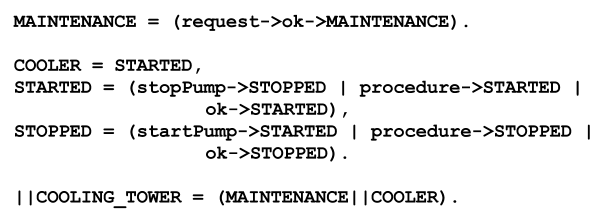
\includegraphics[scale=0.50]{img/FSP.png}
    \caption{Ejemplo FSP}
    \label{FSP}
\end{figure}

A su vez, los FSP soportan distintos operadores de composición como la composición en paralelo. Dicha operación,
denotada como $|\ |$, está definida para preservar la semántica de la composición en paralelo de los LTS definidos en la
definición \ref{COMP_EN_PARALELO}. Por lo tanto, dados dos procesos FSP \texttt{P} y \texttt{Q}, tenemos:
\texttt{lts(P||Q) = lts(P)||lts(Q)}.

Los procesos FSP que están definidos mediante una composición de dos procesos no auxiliares, son llamados procesos
compuestos y sus nombres poseen el prefijo $|\ |$. En nuestro ejemplo, la composición en paralelo entre los procesos FSP 
\texttt{\textbf{MAINTENANCE}} y \texttt{\textbf{COOLER}} se escribe como \texttt{\textbf{||COOLING\_TOWER =
(MAINTENANCE||COOLER).}}

Además, FSP posee palabras reservadas que se colocan antes de la definición de un proceso que fuerzan a la herramienta
MTSA a realizar una operación más compleja al proceso. Un caso de estos, es la palabra reservada
\texttt{\textbf{minimal}}, la cual, hace que MTSA construya un LTS minimal que respeta la semántica equivalente o la
palabra reservada \texttt{\textbf{deterministic}}, que construye un LTS minimal con respecto a las trazas.

FSP también permite definir propiedades FLTL. Un fluent que marca aquellos estados donde la bomba está apagada puede ser
expresada en lenguaje FSP mediante el siguiente código: \texttt{\textbf{fluent IsStopped = <stopPump,startPump>\ initially 0}}.
Como dijimos anteriormente, la bomba empieza encendida, por lo tanto IsStopped es inicialmente falso, pasa a ser
verdadero cuando sucede la acción \texttt{\textbf{stopPump}} y falso nuevamente cuando la acción \texttt{\textbf{startPump}} sucede.

Finalizando, FSP nos otorga facilidad para especificar LTSs y FLTL fórmulas. Este lenguaje es el que utilizaremos en los
siguiente capítulos para definir modelos que representan ambientes y objetivos. 


\chapter{MTSA como herramienta de modelado y síntesis}
\label{MTSA_tool}

En este capítulo reportaremos los casos de estudio que corrimos para validar nuestro enfoque. El propósito de los casos
de estudio es mostrar la aplicación del enfoque mediante la resolución de casos de estudios tomados de trabajos previos
y a su vez, seguir analizando las virtudes y defectos de los trabajos previos existentes de actualización dinámica de
controladores.

\begin{figure}
\centering
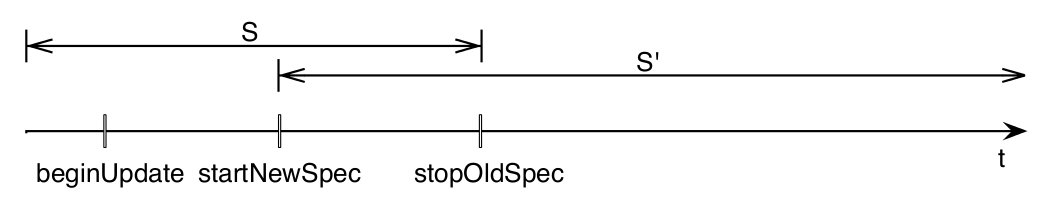
\includegraphics[scale=0.35]{img/overlaping.png}
\caption{Abstracción de la linea de tiempo de la actualización dinámica de controladores. Escenario en el cual la nueva
especificación está garantizada antes de que la vieja especificación deje de valer.}
\label{overlaping}
\end{figure}

\begin{figure}
\centering
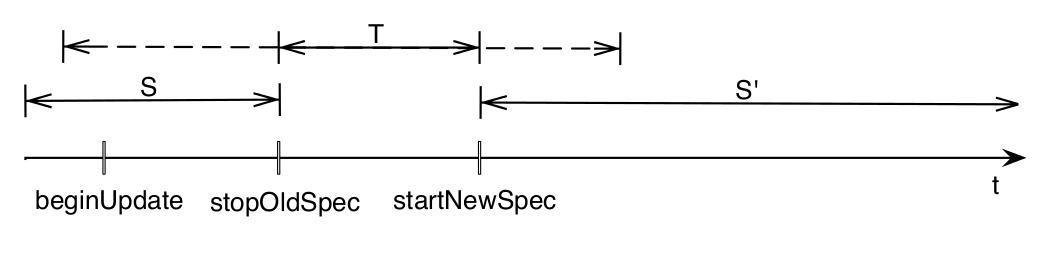
\includegraphics[scale=0.35]{img/transition.png}
\caption{Abstracción de la linea de tiempo de la actualización dinámica de controladores. Escenario en el cual hay un
periodo donde ni la vieja, ni la nueva especificación vale.}
\label{transition}
\end{figure}

Según nuestro conocimiento, el primer y único trabajo que investiga sobre actualización dinámica de controladores donde
hay un cambio de especificación explícito es en Ghezzi et al. \cite{6224401}. Ellos adoptan un criterio general,
natural y correcto. Una actualización dinámica es correcta si el comportamiento exhibido por el sistema es equivalente
al obtenido luego de una actualización apagando la máquina. Esto relaja el esfuerzo del ingeniero al no tener que
especificar requerimientos de transición (como en nuestro trabajo) pero con el costo de limitar posibles actualizaciones
que pueden ser soportadas. Como en \cite{6224401}, permitimos especificaciones solapadas (ver Figura \ref{overlaping}); pero
también permitimos periodos en los que ninguna especificación vale a diferencia de \cite{6224401} (ver Figura
\ref{transition}).

Es posible obtener el comportamiento de actualización obtenido en \cite{6224401} especificando como parte del
requerimiento de transición $T$ que $startNewSpec$ pueda ocurrir si la nueva especificación vale desde el último estado
inicial antes de $beginUpdate$ (ver la imagen de abajo de la Figura \ref{ghezzi}) o tan pronto como el estado inicial es
alcanzado nuevamente (ver la imagen de arriba de la Figura \ref{ghezzi}). Esto, podemos formalizarlo de la siguiente manera:

\vspace{-1cm}
\begin{equation}
\label{ghezzi_formula}
\Box [(LastInitBeforeUpdate \wedge G'\ W\ startNewSpec) \lor (startNewSpec \Longrightarrow Init)]
\end{equation}
\noindent donde $LastInitBeforeUpdate = Init \wedge \bigcirc(\neg Init\ W\ beginUpdate)$ y $Init$ representa estar en un estado inicial de
$C$.

En \cite{PanzicaLaManna:2013:FCC:2487336.2487349}, tres criterios de actualización mas débiles son introducidos para
permitir actualizaciones en sistemas donde el estado inicial no es visitado nuevamente. Por ejemplo, la noción de
estados co-inicial (estados que son similares al estado inicial), expande las situaciones en las cuales la actualización
es permitida. De todos modos, no hay garantías, para ninguno de los nuevos criterios, que el criterio correcto original
si tiene. La falta de garantías requiere de un ingeniero que valide el controlador resultante. En nuestro trabajo,
involucramos a un ingeniero capacitado y habilitado para proveer una especificación de un criterio correcto para la
actualización ($T$).

\begin{figure}[H]
\centering
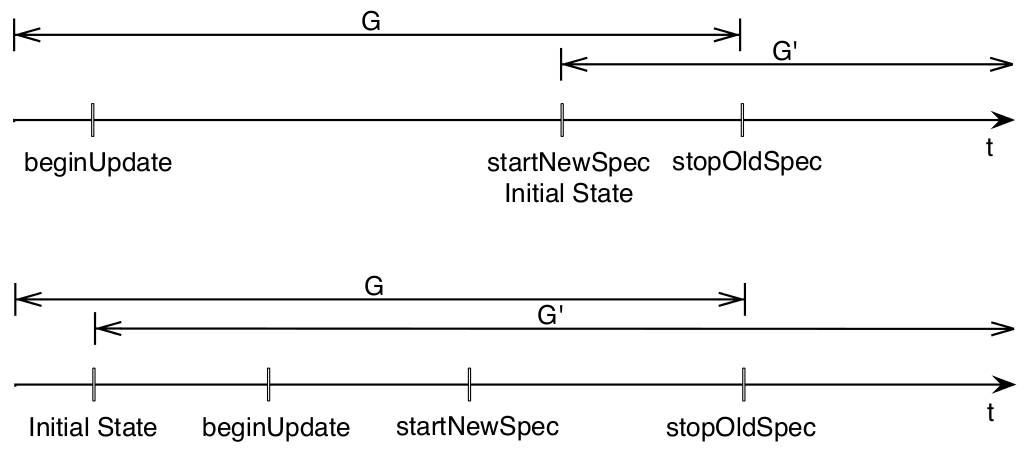
\includegraphics[scale=0.35]{img/Ghezzi.png}
\caption{Relación de eventos relevantes en la actualización de controladores dinámicamente para estados actualizables
según \cite{6224401}}
\label{ghezzi}
\end{figure}


\section{Construcción}

En MTSA, los modelos son definidos mediante una extensión del lenguaje de Procesos de Estados Finitos (FSP). Dicho
lenguaje es un lenguaje textual centrado en la construcción composicional de modelos complejos que originalmente fue
usado para describir LTSs.

Los FSP incluyen varios operadores tradicionales para describir modelos de comportamiento, de los cuales destacaremos el
prefijo de acción ($\rightarrow$), elección ($|$), composición paralela ($\|$) y mezcla.
La semántica de la mezcla es tal que dada dos descripciones parciales del mismo componente, el operador de mezcla
devuelve una LTS que combina la información provista por las descripciones parciales originales.

Es necesario destacar que construir los modelos que son compuestos sigue siendo una tarea dificultosa que requiere de un
intenso trabajo y un grado considerable de experiencia. Para mitigar este problema, MTSA también provee la funcionalidad
que permite sintetizar modelos de comportamiento de forma automática, a partir de especificaciones declarativas de los
requerimientos, escenarios y casos de uso.

La palabra clave \emph{constraint} de MTSA se usa de manera conjunta con las propiedades de seguridad (\emph{safety}) y
se formalizan haciendo uso de la Lógica Lineal Temporal de Fluents (FLTL). Para una declaración de tipo \emph{constraint},
MTSA construye automáticamente el modelo de LTS que caracteriza a todos los modelos LTS libres de \emph{deadlock} que
satisfacen la fórmula FLTL. Al sintetizar y mezclar modelos LTS obtenidos con definiciones FLTL, se puede construir de
forma iterativa un LTS que caracteriza a la cota superior de los sistemas de comportamiento esperados.

La palabra clave \emph{abstract} de MTSA puede aplicarse a procesos FSP. Su semántica es tal que el modelo resultante es
el LTS de menor refinamiento que garantiza el comportamiento requerido por los procesos FSP. Esta palabra clave,
utilizada en conjunción con los procesos FSP que modelan el comportamiento descripto en la especificación del escenario,
provee una LTS que caracteriza a todas las implementaciones que satisfacen dicha especificación.

\section{Análisis}

Habiendo construido una aproximación inicial del comportamiento esperado del sistema, el análisis pasa a ser una tarea
crucial que puede brindar información del dominio tanto del problema como de la solución, aumentando la confianza que se
tiene de la adecuación y correctitud del software y llama a proseguir la elaboración del modelo parcial. 

MTSA soporta varios tipos de análisis, el más básico involucra la inspección de modelos LTS y está soportado a través de
la construcción automática de representaciones visuales de los modelos LTS escritos usando FSP. Esta inspección queda
sujeta al tamaño del modelo, limitación tal que puede mitigarse haciendo uso de los operadores de minimización y
ocultamiento.

Aunque la inspección y animación no permiten una exploración exhaustiva de los modelos LTS, MTSA implementa un número de
técnicas de análisis automáticas para éste propósito. En particular, MTSA permite verificar si un modelo LTS satisface
una propiedad expresada en FLTL. Un modelo LTS caracteriza un conjunto de implementaciones, de las cuales algunas pueden
satisfacer la propiedad siendo verificada y algunas pueden violarla. Por este motivo MTSA automáticamente verifica una
relación de satisfactibilidad trivaluada entre el modelo LTS y una fórmula FLTL. Mientras que un Modelo LTS $M$ puede
caracterizar a un conjunto extremadamente grande, potencialmente infinito, de implementaciones, verificar una propiedad
en $M$ con emph{model checking} se reduce a dos verificaciones tradicionales de FLTL. Finalmente, MTSA permite verificar si un
modelo es libre de \emph{deadlocks}. Al igual que en el caso de \emph{model checking} para propiedades FLTL, el
resultado de esta verificación tiene uno de tres valores: o bien todas las implementaciones exhiben \emph{deadlocks}, o
bien todas son libres de \emph{deadlocks} o bien hay una combinación de implementaciones que exhiben \emph{deadlocks} y
otras que no.

\section{Modelando objetivos para controladores actualizables}

Agregamos un conjunto de palabras reservadas a FSP para poder soportar objetivos actualizables. En la figura
\ref{TEMPLATE1} mostramos el código FSP necesario para síntesis de controladores actualizables para el ejemplo del reactor nuclear
presentado en la sección \ref{}.

El operador \texttt{\textbf{updatingController}} devuelve, si existe, un controlador que satisface una especificación
acerca de los nuevos requerimientos. Necesitamos en esta declaración, además de los nuevos requerimientos, suministrar
la información necesaria acerca de cual es el controlador actual, el modelo del ambiente actual, el modelo del ambiente
nuevo y un conjunto de pares de flujos donde cada elemento indicará correspondencia de estados del ambiente actual al
ambiente nuevo como dijimos en la sección \ref{}. Por ejemplo, en la figura \ref{TEMPLATE1} podemos observar que
al usar la palabra reservada \texttt{\textbf{updatingController}} configuramos BLA1 como el controlador actual, BLA2
como modelo del ambiente actual, BLA3 como modelo del ambiente nuevo, \texttt{\textbf{UpdateSpec}} como la nueva
especificación y \texttt{\textbf{\{\{RequestPending,RequestPending\}, \{IsStopped,IsStopped\}\}}} es el conjunto de
flujos.

Los objetivos nuevos están definidos mediante el operador \texttt{\textbf{controllerSpec}}. La palabra reservada
\texttt{\textbf{safety}} permite definir requerimientos de seguridad (\emph{safety}). Aquí incluiremos las formulas
LTL descritas en la sección \ref{}

La sección de \emph{liveness} esta definida ... 


\chapter{Problema de controladores actualizables dinámicamente}
\label{updating_controller_chapter}

En este capítulo reportaremos los casos de estudio que corrimos para validar nuestro enfoque. El propósito de los casos
de estudio es mostrar la aplicación del enfoque mediante la resolución de casos de estudios tomados de trabajos previos
y a su vez, seguir analizando las virtudes y defectos de los trabajos previos existentes de actualización dinámica de
controladores.

\begin{figure}
\centering
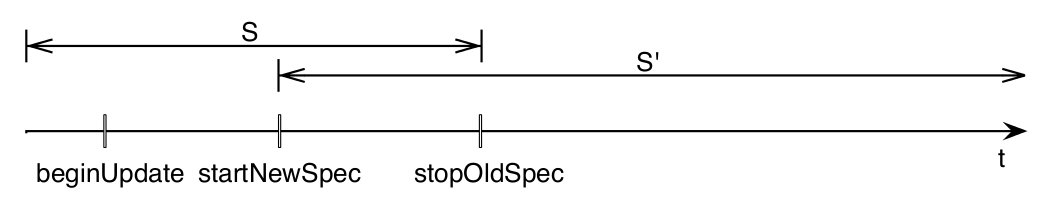
\includegraphics[scale=0.35]{img/overlaping.png}
\caption{Abstracción de la linea de tiempo de la actualización dinámica de controladores. Escenario en el cual la nueva
especificación está garantizada antes de que la vieja especificación deje de valer.}
\label{overlaping}
\end{figure}

\begin{figure}
\centering
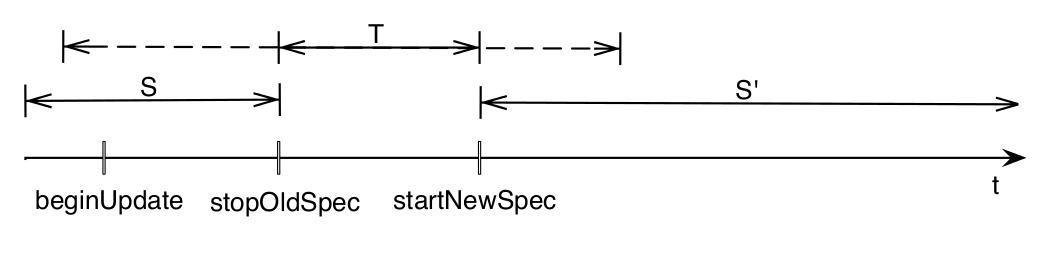
\includegraphics[scale=0.35]{img/transition.png}
\caption{Abstracción de la linea de tiempo de la actualización dinámica de controladores. Escenario en el cual hay un
periodo donde ni la vieja, ni la nueva especificación vale.}
\label{transition}
\end{figure}

Según nuestro conocimiento, el primer y único trabajo que investiga sobre actualización dinámica de controladores donde
hay un cambio de especificación explícito es en Ghezzi et al. \cite{6224401}. Ellos adoptan un criterio general,
natural y correcto. Una actualización dinámica es correcta si el comportamiento exhibido por el sistema es equivalente
al obtenido luego de una actualización apagando la máquina. Esto relaja el esfuerzo del ingeniero al no tener que
especificar requerimientos de transición (como en nuestro trabajo) pero con el costo de limitar posibles actualizaciones
que pueden ser soportadas. Como en \cite{6224401}, permitimos especificaciones solapadas (ver Figura \ref{overlaping}); pero
también permitimos periodos en los que ninguna especificación vale a diferencia de \cite{6224401} (ver Figura
\ref{transition}).

Es posible obtener el comportamiento de actualización obtenido en \cite{6224401} especificando como parte del
requerimiento de transición $T$ que $startNewSpec$ pueda ocurrir si la nueva especificación vale desde el último estado
inicial antes de $beginUpdate$ (ver la imagen de abajo de la Figura \ref{ghezzi}) o tan pronto como el estado inicial es
alcanzado nuevamente (ver la imagen de arriba de la Figura \ref{ghezzi}). Esto, podemos formalizarlo de la siguiente manera:

\vspace{-1cm}
\begin{equation}
\label{ghezzi_formula}
\Box [(LastInitBeforeUpdate \wedge G'\ W\ startNewSpec) \lor (startNewSpec \Longrightarrow Init)]
\end{equation}
\noindent donde $LastInitBeforeUpdate = Init \wedge \bigcirc(\neg Init\ W\ beginUpdate)$ y $Init$ representa estar en un estado inicial de
$C$.

En \cite{PanzicaLaManna:2013:FCC:2487336.2487349}, tres criterios de actualización mas débiles son introducidos para
permitir actualizaciones en sistemas donde el estado inicial no es visitado nuevamente. Por ejemplo, la noción de
estados co-inicial (estados que son similares al estado inicial), expande las situaciones en las cuales la actualización
es permitida. De todos modos, no hay garantías, para ninguno de los nuevos criterios, que el criterio correcto original
si tiene. La falta de garantías requiere de un ingeniero que valide el controlador resultante. En nuestro trabajo,
involucramos a un ingeniero capacitado y habilitado para proveer una especificación de un criterio correcto para la
actualización ($T$).

\begin{figure}[H]
\centering
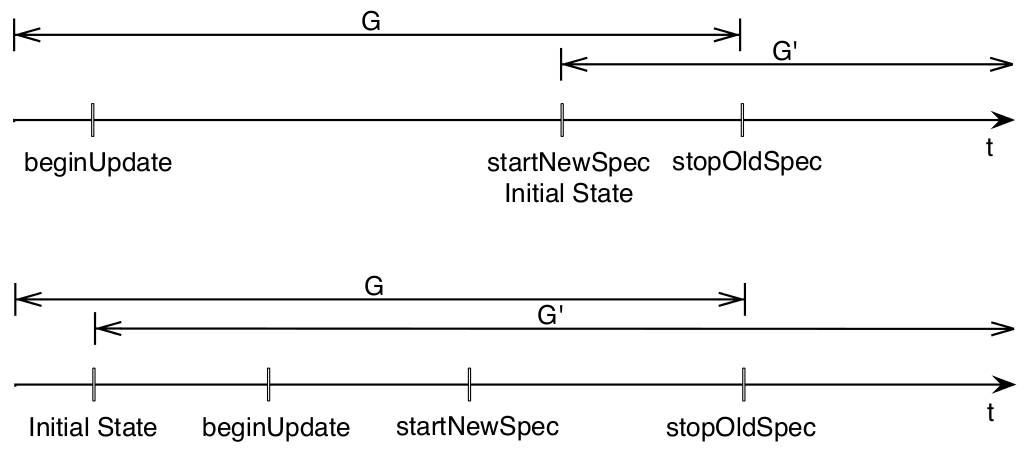
\includegraphics[scale=0.35]{img/Ghezzi.png}
\caption{Relación de eventos relevantes en la actualización de controladores dinámicamente para estados actualizables
según \cite{6224401}}
\label{ghezzi}
\end{figure}


\section{Especificación}

En capítulos anteriores mostramos ejemplos en los cuales nos referíamos a la actual y nueva especificación como
entidades monolíticas (las llamaremos $S$ y $S'$ respectivamente). Sin embargo, para presentar la actualización dinámica
de controladores como un problema de control asumiremos que la especificación $S$ esta dividida en tres partes. La
primera es la descripción de la interfaz del controlador dada como un conjunto de etiquetas $A$ que representa las
acciones controlables del controlador. La segunda es una descripción operacional $E$, en forma de LTS, que describe el
comportamiento del ambiente en cuanto a acciones controlables y monitoriables. La tercera son los objetivos del
controlador $G$, expresado como una formula FLTL.

Tenga en cuenta que como el estado inicial de $E'$ depende el estado actual de $E$, el ingeniero debe proveer un mapeo de estados
$M$ de $E$ a $E'$. Omitiremos referirnos a $M$ hasta que lleguemos a la sección donde formalizaremos todos estos
conceptos para mantener la presentación simple.

En consecuencia, el problema general que apuntamos a resolver puede ser planteado de la siguiente manera: Ejecutar
un sistema adaptable mediante un controlador $C$ que controla un conjunto de acciones $A$ y a su vez satisface los
objetivos $G$ para un ambiente $E$. El usuario desea cambiar dinámicamente el controlador que se esta ejecutando para
empezar a satisfacer el nuevo objetivo $G'$ en el nuevo ambiente $E'$ controlando un conjunto de acciones $A'$ y a su
vez satisfacer los requerimientos de transición $T$.

METER ALGÚN EJEMPLO

Los modelos de los ambientes $E$ y $E'$ pueden ser construidos mediante la composición paralela de varios modelos LTSs
que describen diferentes aspectos del comportamiento del ambiente. Por ejemplo podríamos definir una LTS que describa el
comportamiento de un tren que va atravesando distintas secciones de una vía. Por otro lado, tenemos otra LTS que
describe la comunicación que el tren realiza con la barrera electrónica para identificar si está habilitado para cruzar.
Para definir por completo el ambiente, necesitamos componer en paralelo ambas LTS. El comportamiento del ambiente por
completo puede verse en la sección de casos de estudio.

NECESITO EL EJEMPLO

\section{La actualización dinámica de controladores como un problema de síntesis de controladores}

Una primera aproximación intuitiva para implementar la actualización de controladores dinámicamente puede ser
construyendo dos controladores adicionales al controlador actual $C$. El primero es un controlador $C'$ que puede
satisfacer los objetivos $G'$ para el nuevo ambiente $E'$ controlando acciones $A'$. El segundo es un ``controlador de
transición'' $C^*$ que controla el traspaso del controlador actual $C$ al nuevo controlador $C'$ satisfaciendo los
requerimientos de transición $T$.

Si bien es conceptualmente elegante, el enfoque de los tres controladores es ingenuo ya que estos controladores están
intrínsecamente relacionados. La nueva especificación sólo puede ser alcanzada por un controlador $C'$ desde estados
específicos ($I_{C'}$). Estos estados iniciales de $C'$ necesitan ser calculados y considerados como estados finales del
``controlador de transición'' $C^*$. Luego, los estados desde donde el ``controlador de transición'' puede alcanzar
$I_{C'}$ necesitan ser computados ($I_{C^*}$). Finalmente, nos queda analizar si $C$ puede ser extendido para
garantizar que alcance algún estado en $I_{C^*}$ sin violar sus objetivos ($G$).

La interacción entre estos tres controladores y la necesidad de generar una técnica para computar $C'$ y $C^*$ puede ser
obtenida mediante la resolución de un problema de control que produce un sólo controlador (el cual vamos a llamar $C_u$)
que ejecuta acciones simulando las tres faces, primero simulando a $C$, luego a $C^*$ y finalmente a $C'$. Ahora
pasaremos a explicar como la actualización de controladores dinámica puede ser expresada como un problema de control que
abarca estas tres fases.

El problema de control para la actualización de controladores dinámicos, como cualquier otro problema de control,
necesita de un modelo del ambiente, el cual llamaremos $E_u$, un objetivo, el cual llamaremos $G_u$, y un conjunto de
acciones, $A_u$. El objetivo $G_u$, lo definiremos en términos de $G$, $G'$ y $T$ más los eventos $stopOldSpec$,
$startNewSpec$ y $beginUpdate$. El ambiente $E_u$ estará definido en base a $E$, $E'$ y $C$. El conjunto de acciones
$A_u$ estará definido en base a $A$ y $A'$.

\subsection{El objetivo del problema de control}

La formalización del objetivo para la actualización de controladores dinámicamente, $G_u$, puede ser formalizado
como una conjunción de las siguientes formulas FLTL.

\begin{nahaDef}
\label{update_goals_def}
\emph{(Objetivo para el problema de control de la actualización de controladores dinámicamente) Sean $\Box\ G$ y $\Box\ G'$
los objetivos actuales y los nuevos para un escenario de actualización de controladores dinámicamente, donde $G$ y $G'$
son una combinación Booleana de flujos y $T$ es una propiedad de safety. Definimos a $G_u$, el objetivo para el
problema de control de la actualización de controladores dinámicamente como la conjunción de las siguientes fórmulas
FLTL:}

\begin{enumerate}
\itemsep-4mm
\item $(G\ W stopOldSpec)$
\item $\Box(startNewSpec \Longrightarrow \Box G')$
\item $\Box\ T$
\item $\Box(beginUpdate \Longrightarrow \Diamond startNewSpec)$
\item $\Box(beginUpdate \Longrightarrow \Diamond stopOldSpec)$
\end{enumerate}
\end{nahaDef}

La primer fórmula requiere que los objetivos viejo $G$ valgan hasta que el controlador active la señal $stopOldSpec$.
Tenga en cuenta que, esta propiedad de manera aislada significa que la especificación vieja, cualesquiera sean sus estados,
puede dejar de valer en cualquier momento. Esto no es lo deseado para una actualización dinámica, por lo tanto debemos
restringirlo en la especificación de transición ($T$).

La segunda fórmula simplemente requiere que la nueva especificación empiece a valer desde el momento en que el
controlador active la señal $startNewSpec$. Esto forzará al controlador a que sólo produzca esta señal cuando puede
asegurar $G'$.

La tercera fórmula indica que los requerimientos de transición deben valer siempre. Restringimos $T$ a que sea una
propiedad de seguridad (\emph{safety}). $T$ es esperado que predique sobre eventos $stopOldSpec$ y $startNewSpec$ para
poder restringir el comportamiento del sistema cuando ni $G$ ni $G'$ valen. Un enfoque más preciso sería requerir que
$T$ sólo valga entre ambos eventos, esto seria $\Box inTransition \Longrightarrow T$ donde $inTransition =
\langle\{stopOldSpec\},\{startNewSpec\}, \bot\rangle$. Esta idea es muy restrictiva ya que los requerimientos de transición
pueden necesitar referirse a situaciones que suceden antes que la especificación vieja deje de valer. Por ejemplo, en el
caso del buscador UAV de vida salvaje \ref{buscador_UAV}, una foto tomada antes de $stopOldSpec$ que no fue
procesada antes $stopOldSpec$. O puede ser necesario referirse a situaciones que suceden luego de $startNewSpec$. En
nuestro ejemplo no empezar a satisfacer la nueva especificación hasta que todas las fotos sin procesar sean procesadas.

Finalmente, las ultimas dos fórmulas requiere que el controlador luego de ejecutar la acción $beginUpdate$, continúe con
el procedimiento y garantice que los eventos $stopOldSpec$ y $startNewSpec$ sucedan.

\subsection{Modelo del ambiente del problema de control}

El modelo del ambiente $E_u$ para la actualización de controladores dinámicamente debe ser construido para cubrir las
tres fases del controlador a ser sintetizado: el ambiente para la especificación vieja, el ambiente para la nueva
especificación, y el ambiente para la transición. A grandes rasgos, esto significa definir a $E_u$ para que sea una
combinación de $E$ y $E'$ más el agregado de transiciones para los eventos $beginUpdate$, $stopOldSpec$ y
$startNewSpec$. Por otro lado, hay dos problemas que debemos tener en cuenta cuidadosamente a la hora de definir
formalmente $E_u$.

El primer concepto clave que debemos considerar en la construcción de $E_u$ esta relacionado en buscar un ambiente que
permita un hot-swap trasparente del controlador actual con el obtenido por la síntesis. Necesitamos que la actualización
del controlador sea estructuralmente idéntico al controlador actual hasta que la acción $beginUpdate$ suceda. Este
requerimiento es crucial para lograr establecer un mapeo de estados desde el controlador actual a los estados de controlador
actualizable. Esto hace que sea trivial que debemos establecer el estado inicial del nuevo controlador basándonos en el
estado actual del controlador viejo, y luego intercambiar controladores durante la ejecución sin perder información del
estado. De esta manera, el nuevo controlador va a continuar ejecutando exactamente de la misma manera que como lo hacía
el viejo hasta el momento que se inicie el proceso de actualización.

Para lograr esta propiedad en el controlador de actualización definiremos su ambiente en su parte inicial como la
composición paralela del controlador viejo y su ambiente (es decir $E\|C$). Esto apunta a construir un controlador
actualizable que inicialmente ejecutará en un ambiente que ya esta siendo controlado por $C$. Tenga en cuenta que como
no queremos que la actualización se interponga con $C$ antes que $beginUpdate$ suceda, vamos a asegurar que en esta fase
el controlador actualizable no controle nada, sólo monitorea lo que sucede.

Es cuando $beginUpdate$ sucede, que el controlador actualizable debe empezar a tomar medidas e intentar garantizar
la transición correcta para satisfacer la nueva especificación. Es decir que luego de que la actualización es
solicitada necesitamos deshabilitar $C$ y por lo tanto, cambiar de fase del ambiente.

Entonces, el ambiente $E_u$ es construido para ser como $E\|C$ y luego, cuando $beginUpdate$ sucede, empezará a
comportarse como $E$ hasta que la nueva especificación se pueda cumplir, momento en el cual $E_u$ se comportará como
$E'$.

El segundo problema que debemos manejar en la construcción de $E_u$ está relacionado con preservar el estado el estado
del ambiente cuando cambia desde $E$ a $E'$. Esto es, que el estado inicial del modelo del nuevo ambiente al
momento de hacer la actualización debería estar configurado de acuerdo al estado actual del modelo del ambiente viejo.
Por ejemplo en nuestro caso de estudio del buscador UAV de vida salvaje de la sección \ref{buscador_UAV}, si el sistema
está en un estado de batería baja, entonces el estado del modelo del nuevo ambiente debería reflejar esto. Por lo tanto,
lo que es necesario es un mapeo de estados que relacione estados del modelo del ambiente viejo $E$ al nuevo $E'$.

El mapeo desde estados de $E$ a $E'$ puede ser definido de varias maneras, sólo necesitamos que todos los estados de $E$
tengan al menos un estado correspondiente en $E'$. Tenga en cuenta que, permitimos subespecificar la correspondencia de
estados de $E'$ permitiendo, por ejemplo, una evolución no determinística desde un estado cuyo valor de batería es
$\lnot LowBattery$ a un estado donde el valor es $MidBattery$ o $\neg HighBattery$. Durante este capítulo vamos a asumir
una relación de mapping de estados $M \subset S_E \times S_{E'}$ que cubre a todos $S_E$. En la herramienta que
desarrollamos, por conveniencia, definimos el mapeo naturalmente sobre definiciones de flujos: un estado $E$ esta
mapeado a todos los estados de $E'$ que preservan el valor de flujos.

Ahora definiremos formalmente el ambiente $E_u$ para el problema de control de la actualización de controladores
dinámicamente:

\begin{nahaDef}
\emph{(Ambiente para el problema de control de la actualización de controladores dinámicamente) Sean $C$ el controlador
actual, $A$, $E$ y $G$ la especificación actual y $A'$, $E'$ y $G'$ la especificación nueva para el problema de
control de actualiazación, donde $E = (S_E, A_E, \Delta_E, s_{E_0})$ y $E' = (S_{E'}, A_{E'}, \Delta_{E'}, s_{E'_0})$.
Además, sea $M \subset S_E \times S_{E'}$ un mapeo de estados tal que para todo $s \in S_E$ existe un estado $s' \in
{S_E'}$. El ambiente para el problema de control de la actualización de controladores dinámicamente ($E_u$) es un LTS
$(S_u,A_u,\Delta_u,s_u)$ tal que $E_u$ es una unión disjunta de estados en $E\|C$, $E$ y $E'$ (i.e. $E_u = S_{E\|C}
\uplus S_E \uplus S_{E'}$), $s_u = s_{E\|C}$, $A_u = A_E \cup A_{E'} \uplus \bar{\ell}|\ell \in A$ y $\Delta_u$ es la relación más
pequeña que satisface las reglas que siguen a continuación donde $\ell \in A_u$:}

\begin{enumerate}
\label{update_environment_def}
\itemsep-4mm
\renewcommand*\labelenumi{[\theenumi]}
\item si $(s,\ell,s') \in \Delta_{E\|C} \wedge \ell \notin A$ entonces $(s,\ell,s') \in \Delta_u$
\item si $(s,\ell,s') \in \Delta_{E\|C} \wedge \ell \in A$ entonces $(s,\bar{\ell},s') \in \Delta_u$
\item si $(s,t) \in S_{E\|C}$ entonces $((s,t), beginUpdate,s) \in \Delta_u$
\item si $(s,\ell,s') \in \Delta_E$ entonces $(s,\ell,s') \in \Delta_u$
\item si $s \in \Delta_E$ entonces $(s,stopOldSpec,s) \in \Delta_u$
\item si $s \in \Delta_{E'}$ entonces $(s,stopOldSpec,s) \in \Delta_u$
\item si $(s,s') \in M$ entonces $(s,startNewSpec,s') \in \Delta_u$
\item si $(s,\ell,s') \in \Delta_{E'}$ entonces $(s,\ell,s') \in \Delta_u$
\end{enumerate}
\emph{Una representación gráfica informal de $E_u$ esta representado en la figura \ref{update_environment}}
\end{nahaDef}

\begin{figure}
\centering
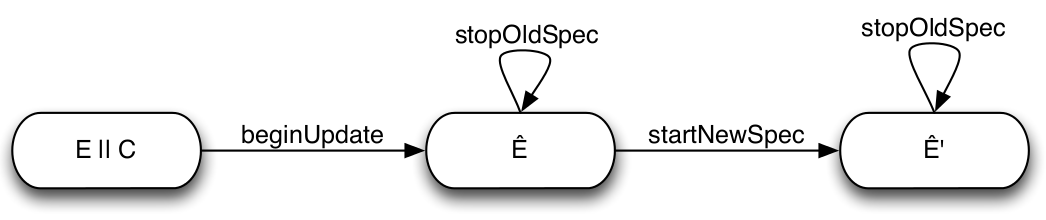
\includegraphics[scale=0.35]{img/E_u.png}
\caption{Representación gráfica del ambiente $E_u$ para el problema de control de la actualización de controladores
dinámicamente - $\hat{E}$ es $E$ con la diferencia de que su estado inicial es el estado actual de $E$ en $E\|C$.
$\hat{E'}$ es $E'$ con la diferencia de que su estado inicial es alguno de los estados relacionados en $M$ con el estado
actual de $E$.}
\label{update_environment}
\end{figure}

Las definiciones anteriores construyen a $E_u$ para comportarse exactamente igual a $E\|C$ (ver reglas 1 y 2) hasta que
sucede $beginUpdate$. La regla 2 simplemente renombra acciones controladas de $C$ para impedir que el controlador de
actualización las controle. Juntas, ambas reglas permiten intercambiar $C$ por $C_u$ mientras aseguramos que $C_u$
continua ejecutando exactamente de la misma manera que $C$. Una vez que $beginUpdate$ se efectua (regla 3), el ambiente
se comporta como $E$ (regla 4). Es justo en este momento que el nuevo controlador tendrá que mantener la vieja
especificación pero forzandolo a llegar a un estado desde el cual los requerimientos de transición puedan ser
satisfechos y luego alcanzar la nueva especificación. En cualquier momento el controlador puede efectuar la acción
$stopOldSpec$ (regla 5) e incluso $startNewSpec$ (regla 7). En caso de que ya haya ocurrido la acción $startNewSpec$, el
ambiente de actualizacion $E_u$ se comporta como el nuevo ambiente $E'$ (regla 8). Aunque como no forzamos que la
vieja especificación deje de valer antes de que valga la nueva especificación, $stopOldSpec$ puede ocurrir durante esta
última fase (regla 6).

\subsection{El problema de control de la actualización de controladores dinámicamente}

Ahora podemos definir formalmente el problema de control que nos soluciona el escenario de la actualización de
controladores dinámicamente.

El problema de control de la actualización de controladores dinámicamente puede ser visto como un problema de control de
LTS usando un ambiente $E_u$ como definimos en la definición \ref{update_environment_def}, los objetivos $G_u$ como
definimos en la definición \ref{update_goals_def} y el conjunto de acciones controlables $A_u$ definido como la unión de las
acciones controlables entre $A$ y $A'$. La única sutileza es que como $E_u$ introduce cambios de nombres de acciones que
son controladas por $C$ en la primera fase ($E\|C$), estos cambios deben ser revertidos una vez computado el controlador
de actualización (reemplazar las acciones $\bar{\ell}$ por $\ell$). Recordar que el cambio de nombre es realizado para
asegurar que el controlador de actualización, cuando se esta generando, no considere a las acciones de $E\|C$ como
controlables hasta que suceda $beginUpdate$. Una vez computado, mientras el controlador de actualización es ejecutado
las acciones deben ser revertidas a su nombre original.

\begin{nahaDef}
\emph{(El problema de control de la actualización de controladores dinámicamente) Sean $G$ y $G'$ expresiones de flujos
sin expresiones temporales. Sea $E$ un LTS y sea la formula FLTL $\Box G$ la especificación actual que el sistema esta
satisfaciendo tras ejecutar el LTS $C$, controlador que controla las acciones en $A$. Sea $E'$ un LTS, la formula FLTL
$\Box G'$ y un conjunto de acciones controlables $A'$ la nueva especificación que es esperada satisfacer con la
actualización dinámica del controlador del sistema.}

\emph{$C_u$ es una solución al problema de control de actualización de controladores dinámicamente si $C_u$ es el resultado de
renombrar toda acción $\bar{\ell}$ por $\ell$ en el controlador $\overline{C}$ que es una solución al problema de
control LTS $\langle E_u, G_u, A_u \rangle$ donde $E_u$ esta definido en la definición \ref{update_environment_def},
$G_u$ esta definido en la definición \ref{update_goals_def} y $A_u = A \cup A'$.}
\label{updating_controller_problem}
\end{nahaDef}

\begin{figure}
\centering
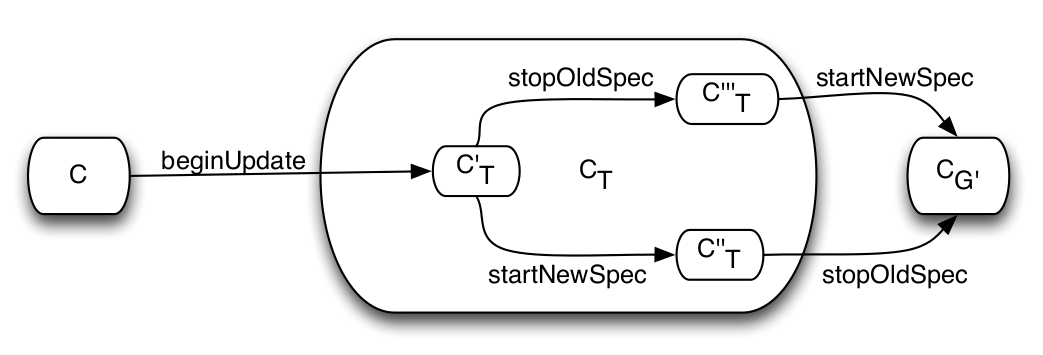
\includegraphics[scale=0.35]{img/C_u.png}
\caption{Abstracción informal de un controlador $C_u$ para el problema de control de la actualización de controladores
dinámicamente - $C_T$ representa el comportamiento que satisface $T$ mientras que garantiza eventualmente tanto
$stopOldSpec$ como $startNewSpec$, mientras que $C_{G'}$ representa el comportamiento del controlador que satisface
$G'$.}
\label{update_controller}
\end{figure}

Por definición, cualquier solución del problema de control de la actualización de controladores dinámicamente
satisfacerá a $G_u$ asumiendo que el ambiente se comporta como $E_u$. La validez de las asunciones de $E_u$ dependen en
la validez de las especificaciones actuales y nuevas, $E$ y $E'$, que son responsabilidad del ingeniero, y que la
infraestructura de ejecución del controlador va a dinámicamente cargar cualquier nueva habilidad descrita en $E'$ cuando
la señal $startNewSpec$ suceda.

Un controlador que es solución del problema definido recientemente tomará, informalmente, la estructura descrita en la
Figura \ref{update_controller}. Primero va a comportarse como $C$ excepto que aceptará en cualquier momento que la acción no controlable
$beginUpdate$ suceda. Luego, se comportará como un controlador que esta intentando realizar las acciones $stopOldSpec$ y
$startNewSpec$ mientras satisface la propiedad $T$. Finalmente, una vez que la acción $startNewSpec$ ha ocurrido se
comportará como un controlador que satisface $G'$.



\section{Resolviendo el problema de actualización dinámica de controladores}

Resolver un problema de control LTS (como el definido en la definición \ref{LTS_control} en el capítulo
\ref{background}) por cada propiedad FLTL es 2EXPTIME complete \cite{Pnueli:1989:SRM:75277.75293}. El problema de
actualización dinámica de controladores es una instancia especifica del problema de control LTS general. En efecto, dada
la estructura de $G_u$, su resolución puede ser computada bajo limites de menor complejidad.

Bajo la asunción de que $G$, $G'$ y $T$ son propiedades de seguridad, $G_u$ puede ser codificado como propiedades de
obligación (por ejemplo disyunciones de afirmaciones de seguridad y alcanzabilidad, $\bigwedge^n_{i=1}(\Box I_i \lor
\Diamond R_i)$). Los problemas de control LTS con objetivos de obligación pueden ser resueltos en tiempo lineal para
modelos de ambientes determinísticos. Para ambientes no determinísticos, un especializado subconjunto de construcciones
pueden usarse para producir versiones determinísticas, sin embargo, podría crecer exponencialmente dependiendo del grado
de no determinismo que exista.

Es simple de ver que el objetivo del problema de control de actualización dinámica de controladores, $G_u$, puede ser
reformulado como afirmaciones de obligación. Las formulas 1) a 3) en la definición \ref{update_goals_def} son propiedades
de seguridad (tenga en cuenta que $W$ es un ``weak until'' y por lo tanto es una propiedad de seguridad). Una propiedad
de seguridad $I_j$ puede simplemente ser codificada como $\Box I_j \lor \Diamond \bot$. Las otras dos formulas de la
definición \ref{update_goals_def} son de la forma $\Box(p \Longrightarrow \Diamond q)$ y pueden ser codificadas como
$\Box \neg UpdateBegan \lor \Diamond (UpdateBegan \wedge NewSpecStarted)$ y $\Box \neg UpdateBegan \lor \Diamond
(UpdateBegan \wedge OldSpecStopped)$ donde los flujos $NewSpecStarted$, $OldSpecStopped$ y $UpdateBegan$ modelan que sus
respectivos eventos han sucedido alguna vez en el pasado. Formalmente estarían definidos como $\langle{startNewSpec},
\emptyset, \bot \rangle$, $\langle{stopOldSpec}, \emptyset, \bot \rangle$ y $\langle{beginUpdate}, \emptyset, \bot
\rangle$.

El problema de control de la actualización dinámica de controladores puede tener o no una solución. La existencia de 
esta solución significa que el controlador resultante $C_u$ garantiza que: se comporte inicialmente como el controlador
actual $C$ bajo la especificación del ambiente actual $E$ y acepta en cualquier punto el comando $beginUpdate$; asegura
una transición correcta, satisfaciendo $T$, preservando el objetivo viejo $G$ y conduciendo al sistema a un punto en el
cual ($startNewSpec$) el nuevo ambiente $E'$ puede ser reemplazado y el nuevo objetivo $G'$ puede ser garantizado.

La no existencia de una solución a este problema de control puede significar dos posibles escenarios. El primero es que
el nuevo objetivo bajo las asunciones del nuevo ambiente no puede ser alcanzados por el controlador (esto es, el
problema de control definido por $E'$ y $\Box G'$ no tiene solución para ningún estado inicial de $E'$). Esta es una
situación extrema donde el controlador tiene poco por hacer con la actualización que se le pide. El segundo, asumiendo
que el problema de control definido por $E'$ y $\Box G'$ tiene solución para algunos estados de $E'$, puede suceder que la
transición de una especificación a la otra no pueda satisfacer la propiedad $T$, o sino puede suceder que sea
imposible alcanzar un estado de $E'$ desde el cual $G'$ valga. Este segundo escenario puede producirse, por ejemplo,
porque el requerimiento de transición $T$ es excesivamente restrictiva o porque el controlador tiene capacidades
insuficientes, para alcanzar un estado desde el cual el nuevo ambiente puede garantizar la validez del nuevo
objetivo. Más generalmente, tendremos el problema cuando tenemos una combinación de especificaciones muy estrictas ($E$,
$G$, $E'$, $G'$ y $T$) y falta de control del controlador sobre los eventos del ambiente.


\chapter{Validación}
\label{validation}

En este capítulo reportaremos los casos de estudio que corrimos para validar nuestro enfoque. El propósito de los casos
de estudio es mostrar la aplicación del enfoque mediante la resolución de casos de estudios tomados de trabajos previos
y a su vez, seguir analizando las virtudes y defectos de los trabajos previos existentes de actualización dinámica de
controladores.

\begin{figure}
\centering
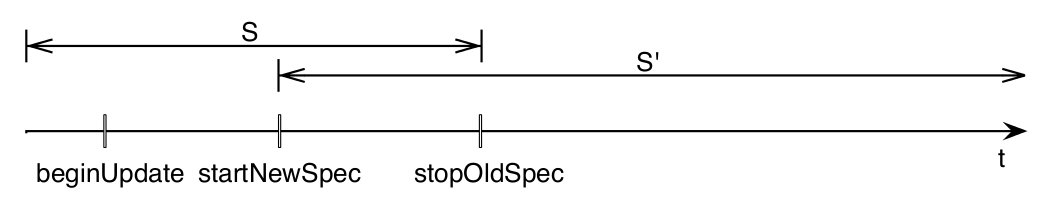
\includegraphics[scale=0.35]{img/overlaping.png}
\caption{Abstracción de la linea de tiempo de la actualización dinámica de controladores. Escenario en el cual la nueva
especificación está garantizada antes de que la vieja especificación deje de valer.}
\label{overlaping}
\end{figure}

\begin{figure}
\centering
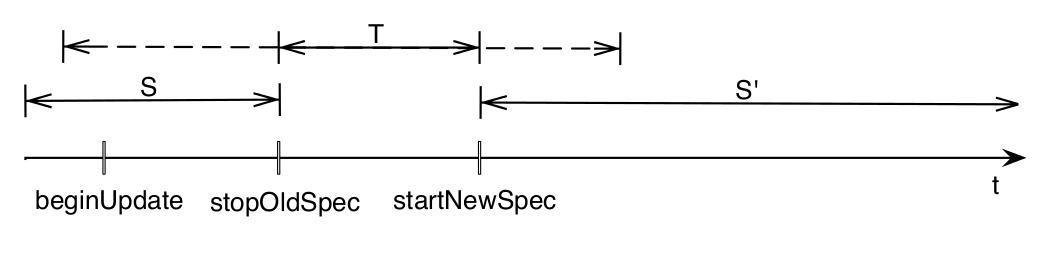
\includegraphics[scale=0.35]{img/transition.png}
\caption{Abstracción de la linea de tiempo de la actualización dinámica de controladores. Escenario en el cual hay un
periodo donde ni la vieja, ni la nueva especificación vale.}
\label{transition}
\end{figure}

Según nuestro conocimiento, el primer y único trabajo que investiga sobre actualización dinámica de controladores donde
hay un cambio de especificación explícito es en Ghezzi et al. \cite{6224401}. Ellos adoptan un criterio general,
natural y correcto. Una actualización dinámica es correcta si el comportamiento exhibido por el sistema es equivalente
al obtenido luego de una actualización apagando la máquina. Esto relaja el esfuerzo del ingeniero al no tener que
especificar requerimientos de transición (como en nuestro trabajo) pero con el costo de limitar posibles actualizaciones
que pueden ser soportadas. Como en \cite{6224401}, permitimos especificaciones solapadas (ver Figura \ref{overlaping}); pero
también permitimos periodos en los que ninguna especificación vale a diferencia de \cite{6224401} (ver Figura
\ref{transition}).

Es posible obtener el comportamiento de actualización obtenido en \cite{6224401} especificando como parte del
requerimiento de transición $T$ que $startNewSpec$ pueda ocurrir si la nueva especificación vale desde el último estado
inicial antes de $beginUpdate$ (ver la imagen de abajo de la Figura \ref{ghezzi}) o tan pronto como el estado inicial es
alcanzado nuevamente (ver la imagen de arriba de la Figura \ref{ghezzi}). Esto, podemos formalizarlo de la siguiente manera:

\vspace{-1cm}
\begin{equation}
\label{ghezzi_formula}
\Box [(LastInitBeforeUpdate \wedge G'\ W\ startNewSpec) \lor (startNewSpec \Longrightarrow Init)]
\end{equation}
\noindent donde $LastInitBeforeUpdate = Init \wedge \bigcirc(\neg Init\ W\ beginUpdate)$ y $Init$ representa estar en un estado inicial de
$C$.

En \cite{PanzicaLaManna:2013:FCC:2487336.2487349}, tres criterios de actualización mas débiles son introducidos para
permitir actualizaciones en sistemas donde el estado inicial no es visitado nuevamente. Por ejemplo, la noción de
estados co-inicial (estados que son similares al estado inicial), expande las situaciones en las cuales la actualización
es permitida. De todos modos, no hay garantías, para ninguno de los nuevos criterios, que el criterio correcto original
si tiene. La falta de garantías requiere de un ingeniero que valide el controlador resultante. En nuestro trabajo,
involucramos a un ingeniero capacitado y habilitado para proveer una especificación de un criterio correcto para la
actualización ($T$).

\begin{figure}[H]
\centering
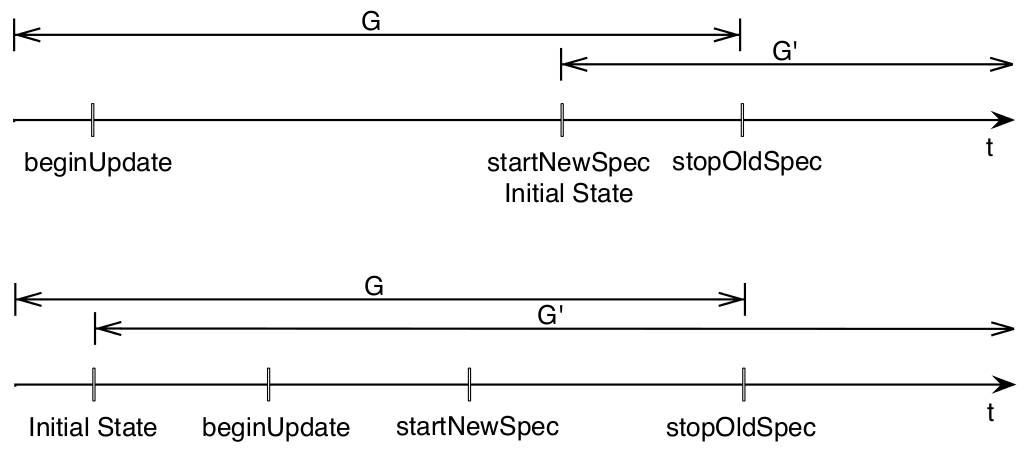
\includegraphics[scale=0.35]{img/Ghezzi.png}
\caption{Relación de eventos relevantes en la actualización de controladores dinámicamente para estados actualizables
según \cite{6224401}}
\label{ghezzi}
\end{figure}


\section{Casos de Estudio}
\label{cases_of_study}

\subsection*{Configuración experimental}

Todos los casos de estudios se ejecutan usando una extensión de la herramienta MTSA \cite{4639371} que nos da soporte
para especificar LTSs y propiedades, usando una notación textual, álgebra de procesos y FLTL. La herramienta también nos 
da soporte para síntesis de controladores para problemas de control SGR(1), los cuales son estrictamente más caros de lo
que es requerido para problemas de control en la actualización de controladores dinámicamente. La herramienta fue 
extendida para automáticamente computar $A_u$, $G_u$ y $E_u$, y resuelve el problema de control de la actualización
dinámica de controladores. La versión extendida de la herramienta y la especificación completa de todos los casos de
estudio pueden verse en \cite{}.

\subsection{Planta de energía nuclear}
\label{power_plant}

En \cite{PanzicaLaManna:2013:FCC:2487336.2487349} se analiza un controlador para un sistema de refrigeración de una
planta de energía nuclear. El controlador actual debe ejecutar servicios de mantenimiento primero apagando la
bomba que refrigera la planta y luego reiniciarla. El nuevo controlador no necesita parar la bomba y reiniciarla para
efectuar el mantenimiento. Hay también un invariante del sistema que indica que la bomba de refrigeración no puede estar
apagada indefinidamente (esto puede llevar a un accidente devastador). 

Los autores muestran que si una actualización se lleva a cabo en un estado en donde el controlador actual tiene la bomba
apagada, entonces el nuevo controlador puede no reiniciar la bomba, generando un accidente. Esto nos muestra dos
problemas. Primero, que la forma segura de preservar el invariante del sistema es requerir que la actualización preserve
el comportamiento como si el controlador actual haya sido reemplazado desde su estado inicial (cuando la bomba es
reiniciada). Esto es lo que los autores aseguran en \cite{6224401}. Segundo, que las restricciones de cuándo una
actualización de \cite{6224401} es suavizada como en \cite{PanzicaLaManna:2013:FCC:2487336.2487349}  puede generar
fallas y consecutivamente ellos recomiendan que ``el diseño de controladores actualizables dinámicamente basados en el
criterio débil de  actualización incluye una subsiguiente validación de los controladores''.

\subsection{RailCab}

El sistema de RailCab es un sistema mecatrónico que fue desarrollado en la Universidad de Paderborn \cite{railcab} donde
los vehículos autónomos deben coordinar de que manera transportar pasajeros o bienes cada vez que le es solicitado. El
sistema que se discute en \cite{6224401} como caso de estudio base es controlar RailCabs cuando está acercándose a un
cruce de vías. El RailCab puede monitorear eventos como $endOfSection$ que determinan que esta entrando a un cruce de
vía, y otros eventos que indican si esta habilitado para usar el freno o si tiene que utilizar el freno de emergencia,
que los llamaremos $lastBrake$ y $lastEmergencyBrake$. El RailCab controla el freno ($brake$) y el freno de emergencia
($emergencyBrake$) e incluso puede recibir respuestas a pedidos que controla como $requestPermissionToEnter$.

La especificación del controlador actual requiere que el RailCab entre al cruce de vías sólo si se le ha garantizado el
permiso para hacerlo. La especificación también describe varias asunciones de que la respuesta al pedido de permiso es
contestada antes de que el RailCab llegue a la sección de $lastEmergencyBrake$, siempre y cuando, el pedido haya sido
realizado antes de llegar a la zona de $lastBrake$. Como ejemplo de una nueva especificación, en \cite{6224401} discuten
hacer un objetivo más fuerte requiriendo que el RailCab envíe otro pedido preguntando si las barreras están funcionando
antes de entrar al cruce de vía. También refuerzan la hipótesis del ambiente en relación a cuando la respuesta a
$checkCrossingStatus$ puede ser recibida.

\subsection{Buscador UAV de vida salvaje}
\label{buscador_UAV}

Este caso de estudio consta de un robot UAV (unmanned aerial vehicle), un típico caso de sistema adaptable, que posee un
controlador para buscar vida salvaje en una área de preservación. El UAV cuenta con un algoritmo de reconocimiento de
vida salvaje que requiere que el UAV vuele en el rango de 40 a 50 metros y trasmita una foto por cada posible objetivo y
debe volver a la base cuando la señal de batería baja se dispara. Durante la misión, se decide que el UAV debe ahora
inmediatamente seguir al primer posible objetivo que encuentre en vez de continuar su búsqueda. Además, deberá trasmitir
una foto de este animal cada 5 minutos. La nueva misión, requiere que el UAV vuele en un rango entre 20 y 30 metros de
altura y use un algoritmo de reconocimiento mejorado. Los módulos del software nuevo van a estar cargados en el UAV y el
controlador debe ser actualizado para lograr sus nuevos objetivos usando los nuevos módulos.

Es importante destacar que los rangos de alturas no solapados implican que un período de transición serán requeridos
entre las dos misiones donde el UAV deberá volar entre 30 a 40 metros de altura y ninguna especificación se satisface.
A su vez, existen otros requerimientos que pueden ser relevantes para el período de transición. Por ejemplo, la nueva
especificación no tiene en cuenta lo que sucederá con las imágenes que están siendo transmitidas por cada animal
encontrado. Consecuentemente, una actualización que sucede entre que un animal es encontrado y la transmisión de la foto
puede llevar a perder la foto. Por lo tanto, un requerimiento para el período de transición puede incluir que a la hora
de dejar de satisfacer la especificación vieja, no haya imágenes pendientes para transmitir.


\subsection{Production Cell}

Consideramos varios escenarios de actualización para el caso de estudio de Production Cell presentado en
\cite{Lewerentz:1995:646391}. El caso de estudio es sobre una fábrica que manofactura diferentes tipos de productos,
donde cada uno de ellos, requiere un proceso de producción que involucra aplicar distintas herramientas en
diferentes ordenes. El sistema de producción de la fábrica debería adaptar su proceso de producción al número de
factores como la cantidad de herramientas disponibles, la especificación de como procesar cada tipo de producto, y otras
restricciones como por ejemplo, un requerimiento de consumo de energía que restringe el uso concurrente de ciertas
herramientas.

Además de las herramientas, la fábrica tiene una bandeja de entrada, una bandeja de salida y un brazo robótico. El brazo
robótico es el encargado de mover los productos entre las herramientas y las bandejas. Los productos en crudo llegan a
la bandeja de entrada, para que el brazo robótico controle cada producto respetando la especificación y colocando el
producto final en la bandeja de salida.

\subsection{Cuadcóptero}

El propósito de este caso de estudio fue experimentar la técnica de actualización dinámica más allá de la especificación
y tareas de síntesis discutidos en los casos de estudio previos. El enfoque, entonces, de este caso es poder analizar un
controlador resultante ejecutando dicha solución en una infraestructura de adaptación (enactment), tomando un dominio de
aplicación especifico. Usamos una infraestructura reportada en \cite{Braberman:2013:CSM:2486788.2487002}, para poder
dinámicamente cargar un controlador en un ARDrone \cite{ARDrone}. La especificación, tanto vieja como nueva, son
simplificaciones del caso de estudio del Buscador UAV de vida salvaje (sección \ref{buscador_UAV}). 

El caso de estudio incluye las acciones de despegar (\emph{takeOff}), aterrizar ($land$), detectar marcas mediante la cámara
onboard ($read$) y objetivos relacionados con las acciones que el drone ejecuta, obteniendo feedback de los leds
onboard, cuando las marcas son leidas ($blink$). La diferencia entre especificación vieja y nueva es que al principio el
robot debe parpadear al leer una marca $x$ y luego de la actualización debe parpadear al leer una marca $x'$ distinta a
la original. Además, luego de la actualización tendremos un contador de batería que irá decrementando su valor a medida
que el ARDrone ejecute acciones. El nivel de batería no debe agotarse nunca para satisfacer los objetivos, y para esto
el robot puede ejecutar la acción $charge$ la que pondrá dicho contador en su nivel más alto.

Por cada una de estas acciones, que son parte de la especificación, definimos una clase $Action$ dentro de nuestro
enactment framework para ejecutar implementaciones del framework YaDrone \cite{YaDrone}.




\section{Resultados}

En esta sección detallaremos los resultados obtenidos para cada caso de estudio planteado en la sección
\ref{cases_of_study}. Para comparar diferentes resultados obtenidos por el problema de control notaremos $Tr(C)$ como el
conjunto de trazas del LTS $C$. Informalmente, una traza es una secuencia de acciones que un controlador puede
realizar. Por lo tanto, dado dos controladores $C_1$, $C_2$, si toda traza de $C_1$ está en $Tr(C_2)$ (i.e. $Tr(C_1)$
$\subset$ $Tr(C_2)$) podremos decir que el controlador $C_2$ tiene más comportamiento que $C_1$ debido a que en el controlador
$C_2$ puedo ejecutar todas las secuencias de acciones de $C_1$ y algunas más.

\subsection{Planta de energía nuclear}

Nosotros resolvemos tres diferentes problemas de control de actualización dinámica de controladores para este caso de
estudio. El primero no tiene requerimientos para el período de transición entre la especificación vieja y la nueva (esto
es, $T$ configurado como $true$). El controlador obtenido ($C^1_u$) exhibe el comportamiento invalido descrito en
\cite{PanzicaLaManna:2013:FCC:2487336.2487349}, permitiendo una actualización mientras la bomba esta apagada, prendiendo
la bomba durante la transición y permitiendo al nuevo controlador a nunca reiniciarla.

El segundo problema de control usa a $T$ con el requerimiento genérico de \cite{6224401} (ver fórmula
\ref{ghezzi_formula}). El controlador resultante ($C_u^{2}$) evita la actualización fuera del estado inicial y en
particular evita la actualización mientras la bomba está apagada. Por otra parte, como se espera, este controlador exhibe
estrictamente menos comportamiento que el controlador previo ($Tr(C^2_u)$ $\subset$ $Tr(C^1_u)$).

Finalmente, el tercer problema de control modela explícitamente el requerimiento de que la bomba no debería estar
apagada continuamente (esto es, en realidad, un requerimiento de transición de aceptación Büchi que puede ser manejado
por nuestro enfoque sin problemas. Ver capítulo \ref{discusion}). El controlador resultante ($C^3_u$) no sólo evita el
escenario descrito en \cite{PanzicaLaManna:2013:FCC:2487336.2487349} y exhibe menos comportamiento que el primer
controlador ($Tr(C^2_u) \subset Tr(C^1_u)$) sino que también provee más oportunidades de actualización que el segundo
controlador exhibiendo estrictamente más comportamiento ($Tr(C^2_u)$ $\subset$ $Tr(C^3_u)$). 

En otras palabras, nuestra técnica provee un criterio más relajado para controladores actualizables con respecto a
\cite{6224401} y que a su vez, es correcto por construcción ya que satisface los requerimientos de transición y además
no necesita de una validación manual posterior como en \cite{PanzicaLaManna:2013:FCC:2487336.2487349}.

\subsection{RailCab}

Como en el caso de estudio previo, resolvimos tres problemas de control de actualización dinámica distintos. El primero
sin requerimientos para la transición entre la vieja especificación y la nueva (i.e. $T = true$). El controlador
resultante $C^1_u$

\subsection{Buscador UAV de vida salvaje}

Utilizamos este caso de estudio, como ejemplo concreto donde no hay salto trivial entre la especificación vieja y la
especificación nueva. Esto se debe a que el UAV en nuestra especificación del problema solo puede volar en tres
posiciones, $high$, $mid$ y $low$, que representan las tres franjas descritas en el caso de estudio. (i.e. entre 40 a 50
metros, entre 30 a 40 metros y entre 20 a 30 metros). Al especificar este problema con nuestra técnica, tendremos que en
conjunto de objetivos $G$, uno de ellos requiere que el UAV vuele en posición $high$. Mientras que en el conjunto de
objetivos $G'$, uno de ellos requiere que el UAV vuele en posición $low$. Esto nos muestra que es necesario hacer
al menos una acción entre $stopOldSpec$ y $startNewSpec$, ya que en caso contrario los objetivos $G'$ nunca podrán ser
asegurados cuando la acción $startNewSpec$ se dispare.

La técnica que definimos en la definición \ref{updating_controller_problem} con $T$ $=$ $true$ nos devuelve un controlador
($C_u^{1}$) que efectúa la acción $low$ entre entre las acciones $stopOldSpec$ y $startOldSpec$ siempre y cuando la
actualización se produzca cuando la misión esta siendo llevada a cabo. De esta manera, la síntesis controla el ambiente
$E$ y lo fuerza a llegar a un estado, donde la actualización es posible. Podemos concluir entonces que el controlador
$C_u^1$ satisface cierta propiedad de manera implícita y sólo realizará la actualización si dicha propiedad vale.

El paso siguiente, en nuestro análisis, fue escribir en FLTL la fórmula implícita que el controlador $C_u^1$ está
satisfaciendo. Por lo tanto, definimos $T$ de la siguiente manera: $T = \Box\ (startNewSpec$
$\rightarrow$ $(FlyingLow$ $||$ $!$ $HeightSet$ $))$ donde $FlyingLow$ y $HeightSet$ son flujos definidos de la siguiente manera: 

\begin{itemize}
\itemsep-4mm
\item $FlyingLow = \langle \{low\},\{high,mid\},\bot\rangle$.
\item $HeightSet = \langle \{high,mid,low\},\{return2base\},\bot\rangle$
\end{itemize}

Mediante esta fórmula FLTL estamos pidiendo que el controlador resultante, luego de la síntesis, cumpla con la propiedad
de que la acción $startNewSpec$ sea disparada, sólo si en ese momento el flujo $FlyingLow$ esta prendido o $HeighSet$
está apagado, es decir, si el UAV esta volando en la franja de 20 a 30 metros o si está en la base. Al controlador
obtenido con esta propiedad lo llamaremos $C_u^2$ y lo comparamos con el controlador obtenido anteriormente.

Los resultados obtenidos cumple que $Tr(C_u^1)$ $=$ $Tr(C_u^2)$ mostrando que la técnica propuesta en esta tesis logra
adaptarse a situaciones adversas donde, antes de realizar la actualización, el controlador debe primero forzar al
sistema a que ciertas propiedades valgan.

El último controlador que generamos, para este caso de estudio, es un controlador que cumple con el requerimiento genérico
del trabajo de \cite{6224401} (ver fórmula \ref{ghezzi_formula}). El controlador obtenido ($C_u^3$) muestra nuevamente
un controlador con menos comportamiento que los controladores obtenidos anteriormente ($Tr(C_u^3) \subset Tr(C_u^1)$).
Esto se debe a que $C_u^3$ sólo acepta actualizaciones cuando el sistema alcanza un estado inicial (o similares al
inicial). Para este caso de estudio, esos estados son alcanzados cuando el UAV se encuentra en la base. Si bien es
correcto que el sistema se actualice en ese momento, porque el UAV elegirá la altura cuando inicie la misión, con esta
técnica, perdemos la posibilidad de realizar una actualización durante la misión. Estas actualizaciones son
soportadas por la técnica propuesta en este trabajo.

\subsection{Production Cell}

Para analizar este caso de estudio, exploramos varios escenarios de adaptación definiendo una especificación inicial y
nueva. Durante la actualización no se produce un cambio del ambiente pero si de los objetivos. Dicho cambio, consiste en
que los productos deberán ahora ser procesados en otro orden. En un principio, primero debemos usar la agujeriadora y
luego pintar, pero luego de la actualización el orden cambia. 

Estudiaremos durante esta actualización distintos escenarios especificando posibles alternativas. Por ejemplo, una
decisión común para todo escenario de actualización es como son los productos procesados. ?`Debería la cadena de montaje
estar vacía antes de que se produzca la actualización? En este caso, los productos que están siendo procesados al
momento en que la actualización es requerida ?`deberían ser descartados? ?`o terminarlos? Si decidimos terminarlos,
?`los deberíamos terminar con la vieja especificación o con la nueva? O tal vez, durante el proceso de transición, la
cadena de montaje no necesita ser vaciada y no importa que receta se lleva a cabo para construir un producto, siempre y
cuando, estén construidos de una manera consistente. 

Estas alternativas fueron modeladas cambiando el valor del requerimiento de transición $T$ definiéndolo de la siguiente
manera:

\begin{enumerate}
\item $\Box$ $(($ $startNewSpec$ $\rightarrow$ $($ $!$ $Processing['red]$ $\&\&$ $!$ $Processing['yellow]$ $))$ $\&\&$
$($ $stopOldSpec$ $\rightarrow$ $($ $!$ $Processing['red]$ $&&$ $!$ $Processing['yellow]$ $)) )$
\item $\Box$ $($ $startNewSpec$ $\rightarrow$ $StopOldSpec$ $)$
\item $true$
\end{enumerate}

Donde $Processing$ es el flujo que se inicializa cuando un producto entra a la cadena de montaje y se apaga cuando se va
y donde $StopOldSpec$ es el flujo que se prende cuando el evento especial $stopOldSpect$ se ejecuta y no se apaga nunca.

Con la primer fórmula FLTL estamos forzando al sistema a que solo genere la actualización si no hay ningún producto en
la cadena de montaje, de esta forma no ahorramos el problema de tener que decidir qué hacer con los productos que están
pendientes.

Con la fórmula 2, forzamos al sistema a generar actualizaciones sólo cuando la especificación vieja no esta siendo
garantizada. De esta manera, evitamos que ambas especificaciones estén siendo garantizada, lo que sería un problema, ya
que en esta actualización los objetivos actuales y los objetivos nuevos son opuestos (i.e. o bien uso el taladro primero
y luego pinto o bien pinto primero y luego taladro, ambos objetivos no son posibles de satisfacer).

Con la tercer fórmula, estamos dejando a la técnica libre, permitiéndole forzar al sistema a que haga lo que crea
conveniente para satisfacer los objetivos nuevos.

Los resultados obtenidos...

\subsection{Cuadcóptero}

Un aspecto interesante del controlador resultante, en este caso de estudio, es que en la vieja especificación el nivel
de batería nunca es tenido en cuenta, generando en el ambiente de actualización $E_u$ mucho no determinismo a la hora de
efectuar la acción $startNewSpec$ desde cualquier estado de $E$ (i.e. una transición por cada nivel de batería distinto que
puede tener el nuevo ambiente). A pesar del no determinismo que este problema de control tiene al cambiar la
especificación, el controlador de actualización simplemente carga la batería inmediatamente después de que se efectúe la
actualización (i.e. cuando $startNewSpec$ ocurre). Esto sucede debido a que el controlador de actualización obtenido
asume una actualización en el peor caso, que es cuando no hay batería disponible en el robot.

Por otra parte, Pudimos validar el comportamiento del drone tras observar mediante la herramienta MTSA como los estados
del controlador de actualización eran recorridos, y a su vez, observar las acciones reales que el robot efectuaba. La
única acción controlada por el operador del sistema vía MTSA fue $beginUpdate$. Un video con uno de estos experimientos
puede ser visto en \url{https://www.youtube.com/watch?v=dFgFnu9y10M}.




\chapter{Conclusiones y trabajos futuros}
\label{discusion}

\section{Discusión y trabajo futuro}

El problema de actualización dinámica ha sido estudiado extensivamente y hay una gran cantidad de problemas distintos
que deben ser abordados en función del dominio de aplicación, tecnología y la forma en que se efectúa la actualización
(vea \cite{SMR:SMR1556} para mas información). El grueso del esfuerzo en actualización dinámica asume que no hay cambios
de especificación y por lo tanto el mismo comportamiento es esperado (por ejemplo en \cite{mx:icse13}), o que la
especificación es genérica (como en \cite{Shen:2005:TUF:1095430.1081720}, \cite{5551162}, \cite{1167829},
\cite{4221625}, \cite{485222}, \cite{60317}) y no proporcionada por el usuario. Ejemplos de este último, aparte de
asegurar que la actualización no desemboca un fallo, asegura type safety (ej. \cite{Subramanian08dynamicsoftware}) y
data isolation entre versiones \cite{Stoyle07mutatismutandis:}. Quiescence \cite{60317} y nociones relacionadas (ej.
\cite{4359466},  \cite{Anderson:2009:MPM:1656437.1656448}, \cite{485222}) no requieren una representación explicita de
las propiedades a ser preservadas, pero fue utilizado en conjunto con técnicas que garantizan consistencia genérica de
semántica (ej. \cite{5546542}). 

La necesidad de una actualización por medio de la definición de propiedades por parte del usuario han sido reconocidas
en \cite{Baresi:2010:DBD:1882362.1882367}. En \cite{Hayden:2012:SVC:2189314.2189336}, se considera la especificación de
propiedades de actualización, pero posee un enfoque en verificar si el programa satisface estas propiedades, en vez de
automáticamente sintetizar la actualización para satisfacer estas propiedades. 

Síntesis, estrategia operacional para construir un autómata que satisface una especificación dada, ha sido usado
extensivamente para garantizar código que es correcto por construcción (por ejemplo en
\cite{Greenyer:2013:ISC:2491411.2491445}). La naturalidad automática de la síntesis logra poder aplicar esta técnica no
solo en el momento en el que el diseño se lleva a cabo sino que también en tiempo de ejecución, generando una sistema
adaptable. Dicha evolución no esta limitada exclusivamente para sistemas adaptables como describimos en la etapa de
introducción y motivación (ver sección \ref{motivation}). Por ejemplo, en \cite{Pelliccione20082237} el problema de
evolucionar componentes conjuntos es resuelto sintetizando ``glue code'' (por ejemplo, controladores). Si bien la
síntesis se ejecuta sin frenar el sistema, el nuevo controlador solo puede reemplazar al viejo cuando el sistema entra
en ``quiescence''.

Síntesis requiere algún tipo de especificación desde la que, a través de diferentes técnicas de razonamiento, producir
una solución. El resultado de sintetizar es correcto solo en la medida en que la especificación es válida. Por lo tanto,
técnicas de síntesis no son, en principio, resistentes a errores en la especificación o a ambientes que evolucionan y
divergen de la especificación. El trabajo descrito en esta tesis es también susceptible a especificaciones invalidas. En
el dominio de sistemas adaptables se han estudiado distintos enfoques que pueden detectar y resolver ciertas situaciones
(por ejemplo en \cite{DBKMSU14} y \cite{Vromant:2011:ICL:1988008.1988037}) e incluso, aprender nuevas especificaciones
en tiempo de ejecución. El enfoque descrito en este documento puede ser combinada con dichas técnicas.

Una suposición de este trabajo es que es posible controlar cambios del ambiente. En otras palabras, si la nueva
especificación introduce diferentes características en el ambiente, como serían nuevos componentes, cambios en el protocolo
de llamada de un componente, o deshabilitar un componente, es el controlador quien puede decidir cuando estos cambios
ocurren. El controlador controla una infraestructura intermedia que puede cargar, descargar o cambiar componentes en
tiempo de ejecución. Esto permite al controlador a planificar un cambio y darle mas libertad para encontrar una
estrategia que puede satisfacer el cambio requerido. Por otro lado, en muchas situaciones, puede suceder un cambio no
anunciado en el ambiente y actualizar el controlador para acomodar este cambio es decidible.

Por ejemplo, si la conexión entre el UAV y la base puede perderse, y por lo tanto, la interfaz que el controlador de UAV
maneja queda deshabilitado. En este caso, la actualización de este controlador debe producirse inmediatamente y puede
ser imposible continuar garantizando los objetivos actuales o los nuevos. En \cite{DBKMSU14} presentan un enfoque donde las
garantías funcionales del controlador se degradan elegantemente para estos casos. Por otro lado, la técnica requiere que
el controlador y la especificación del nivel de degradación preserve una relación de refinación entre el controlador
actual y la especificación. Dicho requerimiento puede ser restrictivo.

El trabajo realizado en esta tesis, puede ser visto como una generalización de una degradación progresiva presentada en
\cite{DBKMSU14}. Decimos esto, ya que la no controlabilidad del cambio de ambiente, puede en nuestro enfoque manejarse teniendo
que la especificación de transición $T$ requiera que el evento $startNewSpec$ ocurra inmediatamente después de
$beginUpdate$, sin embargo, el ambiente viejo $E$ no es requerido para obtener refinamientos de $E$ como en
\cite{DBKMSU14}

En este trabajo, limitamos la expresividad de nuestro enfoque a objetivos de \emph{safety} (ver Definicion
\ref{update_goals_def}). Esto hace a esta presentación simple e incluso permite una resolución de complejidad lineal al
problema de control de actualización de controladores dinámicamente siempre y cuando el ambiente es determinístico. Sin
embargo, podríamos permitir mayor expresividad en $G$, $G'$ y $T$ sin incurrir del todo en la penalidad de resolver un
problema de control (2EXPTIME-COMPLETE). Es posible, reformular la definición \ref{update_goals_def} para permitir que
las especificaciones $G$, $G'$ y $T$ puedan ser de la forma $\Box \Diamond G$, $\Box \Diamond G'$ y $\Box \Diamond T$.
Este criterio de aceptación de Büchi extiende la expresividad manteniendo la complejidad en orden polinomial (esto lo
conseguimos redefiniendo $G_u$ a $\Box \Diamond [(G \lor OldSpecDropped) \wedge (G' \lor \neg NewSpecEnsured) \wedge
(\neg BeginUpdate \lor NewSpecEnsured) \wedge (\neg BeginUpdate \lor  OldSpecDropped) \wedge  T]$. Donde
$OldSpecDropped$ es el flujo definido como $\langle \{stopOldSpec\},\emptyset,\bot\rangle$, $NewSpecEnsured$ es el flujo
definido como $\langle \{startNewSpec\},\emptyset,\bot\rangle$ y $BeginUpdate$ es el flujo definido como $\langle
\{beginUpdate\},\emptyset,\bot\rangle$). Se necesitan futuras investigaciones para analizar si, por ejemplo, las
especificaciones SGR(1) \cite{D'ippolito:2013:SNE:2430536.2430543} en el problema de control de actualización de
controladores dinámicos, solo puede ser resuelto en tiempo polinómico.


\section{Conclusiones}

Mostramos como resolver el problema de controladores actualizados dinámicamente para satisfacer una nueva especificación
mediante el uso de síntesis de controladores. La solución propuesta garantiza satisfacer la nueva especificación y
cualquier requerimiento de transición que sea dada por el usuario, pero también asegura que la actualización va a
ocurrir tomando el control del sistema bajo la vieja especificación, y forzándolo a un estado seguro desde el cual la
transición puede empezar para garantizar la nueva especificación eventualmente.

Se pueden realizar trabajos futuros cuyo enfoque sería mejorar la expresividad sin pagar el precio de una síntesis
general. También, podríamos hacer la integración con otros enfoques que tienen como objetivo facilitar la capacidad de
adaptación de alto nivel a los sistemas de software complejos. Esto lo lograríamos incluyendo técnicas para aprender el
comportamiento del ambiente en tiempo de ejecución y adaptación cuantitativas para propiedades no-funcionales.




